\documentclass[a4paper,12pt,titlepage]{article}
\usepackage[utf8]{inputenc}
\usepackage[czech]{babel}
\usepackage{amsfonts, amsmath, amsthm, amssymb}
\usepackage[small,compact]{titlesec}
\usepackage{anyfontsize}
\usepackage{rotating}
\usepackage{mdwlist}
\usepackage[left=1.5cm,right=1.5cm,top=1.5cm,bottom=2cm]{geometry}
\usepackage{wrapfig}
\usepackage{subcaption}
\usepackage{hyperref}
\usepackage{color}
\usepackage{tikz}
\newcommand*\circled[1]{\tikz[baseline=(char.base)]{
  \node[shape=circle,draw,inner sep=1pt] (char) {#1};}}

\usepackage{titlesec}
\titleformat*{\section}{\removelastskip\bigskip\LARGE\bfseries}
\titleformat*{\subsection}{\large\bfseries}
\titleformat*{\subsubsection}{\large\bfseries}

\newcommand{\shn}{\Theta}
\newcommand{\lm}{\smallskip\noindent\bf Lemma\rm{} }
\newcommand{\dk}{\smallskip\noindent\bf Důkaz\rm{} }
\newcommand{\df}{\smallskip\noindent\bf Definice\rm{} }
\newcommand{\vt}{\smallskip\noindent\bf Věta\rm{} }
\newcommand{\poz}{\smallskip\noindent\bf Pozorování\rm{} }
\newcommand{\pzn}{\smallskip\noindent\bf Poznámka\rm{} }
\newcommand{\dsl}{\smallskip\noindent\bf Důsledek\rm{} }
\newcommand{\tv}{\smallskip\noindent\bf Tvrzení\rm{} }
\newcommand{\app}{\smallskip\noindent\bf Aplikace\rm{} }
\newcommand{\alg}{\smallskip\noindent\bf Algoritmus\rm{} }
\newcommand{\conj}{\smallskip\noindent\bf Domněnka\rm{} }
\renewcommand{\c}{\mathcal{C}}
\newcommand{\F}{\mathcal{F}}
\newcommand{\B}{\mathcal{B}}
\newcommand{\A}{\mathcal{A}}
\renewcommand{\L}{\mathcal{L}}
\renewcommand{\O}{\mathcal{O}}
\renewcommand{\o}{o}
\newcommand{\E}{\mathbb{E}}
\newcommand{\Z}{\mathbb{Z}}
\newcommand{\C}{\mathbb{C}}
\newcommand{\NP}{\mathcal{NP}}
\newcommand{\R}{\mathbb{R}}
\newcommand{\Q}{\mathbb{Q}}
\newcommand{\N}{\mathbb{N}}
\newcommand{\Ft}{\mathbb{F}}
\newcommand{\xttt}{{\chi_T^\bot}^T}
\newcommand{\todo}[1]{\bf TODO: \rm#1}
\newcommand{\set}[1]{\{#1\}}
\renewcommand{\L}{\mathcal{L}}
\newcommand{\I}{{\bf I}}
\newcommand{\In}{{\bf I}_n}
%\newcommand{\qed}{\hfill QED}
\DeclareMathOperator{\rank}{rank}
\DeclareMathOperator{\disc}{disc}
\DeclareMathOperator{\zz}{\circled{z}}
\DeclareMathOperator{\Sp}{Sp}
\DeclareMathOperator{\Tr}{Tr}
\DeclareMathOperator{\ch}{ch}
\DeclareMathOperator{\Ker}{Ker}
\DeclareMathOperator{\Var}{Var}
\DeclareMathOperator{\girth}{girth}
\DeclareMathOperator{\pcp}{PCP}
\newcommand\bigzero{\makebox(0,0){\text{\huge0}}}
\newcommand\bigone{\makebox(0,0){\text{\huge1}}}
\newcommand{\bigddots}[1]{\makebox(0,0){\rotatebox{-35}{\text{\xleaders\hbox{$\cdot$\hskip4pt}\hskip#1\kern0pt}}}}
\newcommand{\sk}[1]{{\langle #1\rangle}}
\newcommand{\diagdots}[3][-25]{%
  \rotatebox{#1}{\makebox[0pt]{\makebox[#2]{\xleaders\hbox{$\cdot$\hskip#3}\hfill\kern0pt}}}%
}

\title{Státnice -- Informatika -- I4\\ Diskrétní modely a algoritmy\\ ~\\ Kombinatorika a teorie grafů \\ Pravděpodobnostní metody a algoritmy \\ Kombinatorická optimalizace}
\author{Ladislav Láska\\ Jan Musílek}

\begin{document}

\maketitle
\newpage
\tableofcontents
\newpage

\section{Barevnost grafů}

\subsection{Perfektní grafy}

\df (Perfektní graf) Graf je perfektní, pokud pro každý jeho indukovaný podgraf 
platí, že $\chi(G) = \omega(G)$. Některé třídy perfektních grafů jsou:
\begin{itemize}
	\item Bipartitní grafy (pokud obsahují hranu, jsou vždy dvoubarevné).
	\item Chordální grafy (obarvit podle perfektního eliminačního schématu, 
		které nachází maximální kliku).
\end{itemize}

\vt (Lovász) Graf je perfektní právě tehdy, když je jeho doplněk perfektní.

\vt (Berge) Graf je perfektní právě tehdy, když neobsahuje díry (liché cykly) 
ani antidíry (doplňky lichých cyklů) jako indukovaný podgraf.  (Lichý cyklus ani 
doplněk nemůže být perfektní, protože potřebuje 3 barvy, ale má kliku velikosti 
max. 3, opačná implikace je těžká)

\subsection{Barevnost a maximální stupeň}

\vt (Brooksova věta.) Pro souvislý neorientovaný graf $G$ s maximálním stupněm 
$\Delta$ platí, že $\chi(G) \leq \Delta$, pokud nejde o úplný graf nebo lichý 
cyklus (v takovém případě je triviálně $\chi(G) = \Delta+1$.

\dk Indukcí podle velikosti. Pro $n = 1$ platí triviálně.  Předpokládáme 
regulární graf (jinak odebereme vrchol menšího stupně, použijeme indukci a 
vrchol dobarvíme). Pokud je $1$ nebo $2$-souvislý, obarvíme komponenty zvlášť 
indukcí. U 3-souvislého grafu najdeme vrchol s maximálním stupněm $u$, jeho dva 
sousedy $v,w$ nespojené hranou (existují pokud není úplný), vytvoříme kostru 
$G-\{v,w\}$ zakořeněnou v $u$, vrcholy $v,w$ dodáme nakonec a obarvíme hladově 
od listů.  Protože každý vrchol až na $u$ má otce v kostře, zbyde na něj
barva. Na $u$ zbyde proto, že $v$ a $w$ mají stejnou barvu.

\vt (Vizingova) Pro libovolný graf $G$ bez smyček a násobných hran platí: 
$\Delta(G) \leq \chi'(G) \leq \Delta(G) +1$, kde $\chi'$ je hranová barevnost.
{\it Důkaz je indukcí podle počtu hran. Pro hranu $e$ se obarví graf $G-e$ a 
	hrana $e$ se dobarví na volnou barvu z obou vrcholů. Pokud taková není, 
hledá se kde prohodit barvy na střídavé cestě.}

\subsection{Barevnost a girth}

\vt (Grötszchova věta.) Každý rovinný graf bez trojúhelníků je 3-obarvitelný.  
{\it Discharging argument: uvažuje se minimální protipříklad, který neobsahuje 
	zakázané (nereducibilní) konfigurace. Přiřazením záporného náboje a 
distribucí za předpokladu, že konfigurace nejsou obsaženy se získá kladný náboj, 
a to je spor.}.

% MAT307
\vt (O vztahu barevnosti a girth.) Pro každé $k$ a $l$ existuje graf s 
chromatickým číslem $> k$ a girth $>l$. Speciálně omezením girth nezískáme málo 
barevné grafy.

\dk {\it (pouze pro grafy bez trojúhelníků, obecný důkaz v pravděpobnostních
metodách)} Začneme s hranou, to jest $G_2$ (potřebuje 2 barvy).  Vybudujeme
$G_{n+1}$ tak, že přidáme nový vrchol $z$, zdvojíme všechny vrcholy, kopie
spojíme hranou se sousedy svých předloh a $z$.  Takový graf je bez trojúhelníků,
které mohly vzniknout jenom se $z$ a žádní sousedi $z$ nemají mezi sebou hranu
(konstrukce na obrázku \ref{triangle-free-colorful-construction}).  Protože obě
části vrcholů lze obarvit stejně, triviálně umíme obarvit graf $n+1$ barvami.
Předpokládejme, že $G_n$ potřeboval $n$ barev.  Potom pro každou barvu $c$
existuje vrchol, který ji má vynucenou v $G_n$; jeho klon ji ale má vynucenou v
$G_{n+1}$ také, protože sdílí sousedy -- nelze ji tedy využít pro obarvení $z$.
\begin{figure}[h!]
	\centering
	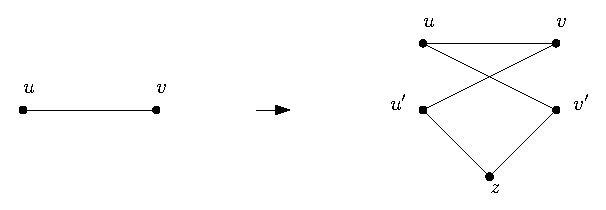
\includegraphics{img/triangle-free-colorful-construction.eps}
	\caption{Postup od $G_2$ na $G_3$}
	\label{triangle-free-colorful-construction}
\end{figure}

\subsection{Vybíravost}

\df (Barvení ze seznamů) Graf je obarvitelný ze seznamů $S_v$ povolených barev 
pro každý vrchol, pokud lze vybrat pro každý vrchol barvu z jeho seznamu 
takovou, že sousední vrcholy mají různou barvu.

\df (Vybíravost) Graf je $k$-vybíravý, pokud ho lze obarvit z libovolných
seznamů délky
$k$, značíme $\ch(G) = k$.

\poz Barevnost je speciální případ vybíravosti, speciálně když jsou všechny
seznamy stejné.

\vt (Thomassen) Každý rovinný graf je 5-vybíravý.

\dk Zavedeme indukční předpoklad: 

{\it Pro rovinný graf $G$, který se skládá z vnějšího cyklu $C$, na kterém jsou 
	dva sousední vrcholy předbarvené, a vnitřní stěny jsou triangulace, lze 
	rozšířit toto předbarvení na celý graf pokud všechny vrcholy na $C$ mají 
seznam délky alespoň $3$ a všechny vnitřní vrcholy alespoň $5$.}

Graf tedy doplníme na triangulaci, určíme vnější stěnu a hodíme graf do indukce 
podle počtu vrcholů. Pokud má graf chordu, rozdělíme ho podle ní na dvě 
poloviny, aplikujeme indukci na každou zvlášť, nejdříve však na půlku, která má 
předbarvené vrcholy. Pokud chordu nemá: předpokládáme $C=\{v_1, \dots, v_k\}$ 
vrcholy na vnější stěně, $v_1$ a $v_2$ jsou již obarvené, obarvíme $v_k$: 
zvolíme dvě barvy ze seznamu $v_k$, vyškrtáme
je z jeho sousedů uvnitř grafu $u_i$ (ti měli 5, zbydou jim alespoň 3, tak 
akorát do indukce) a graf pustíme dál do indukce bez $v_k$ (viz obrázek).  
Následně obarvíme $v_k$ barvou, kterou nepoužil $v_{k-1}$, takové máme dvě, 
které jsme si vyškrtali ze sousedů $u_i$ kromě $v_{k-1}$!

\noindent
\begin{figure}[h!]
	\centering
	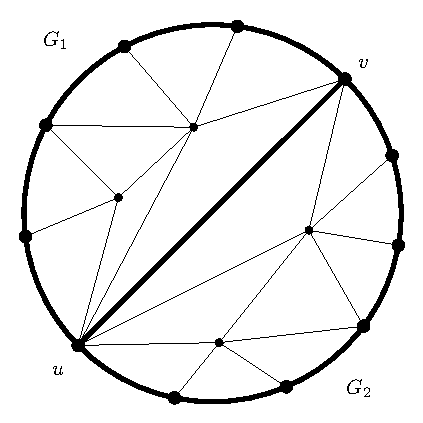
\includegraphics{img/thomassen-chord.eps}
	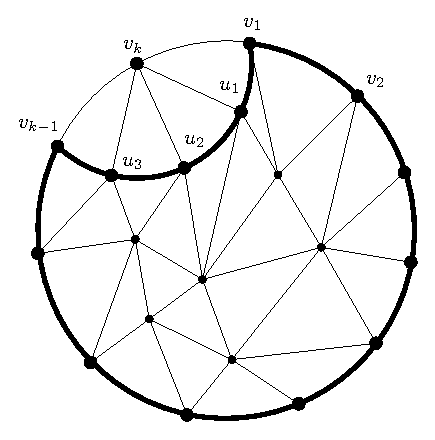
\includegraphics{img/thomassen-induction.eps}
	\caption{Postup indukce v grafu s chordou a bez ní.}
\end{figure}

\df Definujme hranovou barevnost a hranovou vybíravost grafu $G$ jako vrcholovou
barevnost a vybíravost jeho linegrafu, tedy $\L(G)$. Značíme $\chi'(G)$ a
$\ch'(G)$.

\vt (List Coloring Conjecture) Pro každý graf platí $\chi'(G) = ch'(G)$.

\vt (Galvin) Pro každý bipartitní graf platí $\chi'(G) = ch'(G)$.

\subsection{Kernel}

\df (Kernel) Nezávislá množina $U$ v orientovaném grafu je {\it kernel}, pokud 
každý vrchol $v\in G \setminus U$ má hranu $vu$ do nějakého vrcholu $u\in U$.  
{\it Alternativně: každý vrchol je v kernelu, nebo do něj má hranu.}

\lm Nechť $G$ je graf a $D$ jeho orientace a každý vrchol má méně výstupních 
hran, než barev ve svém seznamu, a každý indukovaný podgraf $D$ má kernel, potom
má $G$ seznamové obarvení.

\dk Pro barvu $\alpha$ vezmu graf indukovaný vrcholy, které mají $\alpha$ ve 
svých seznamech. Z předpokladů tento graf má kernel -- obarvím kernel barvou 
$\alpha$, odstraním a pokračuji indukcí (graf se zmenšil, některým vrcholům se 
zmenšily seznamy, ale také ekvivalentně odchozí stupně -- předpoklady stále 
platí).


\section{Regulární grafy}
\df {\it \emph{Regulární graf} je graf, jehož všechny vrcholy mají stejný stupeň. Graf je $k$\emph{-regulární}, je-li stupeň všech jeho vrcholů $k$.}

\begin{itemize*}
\item 0-regulární grafy se skládají z izolovaných vrcholů
\item 1-regulární grafy jsou disjunktním sjednocením hran
\item 2-regulární grafy jsou disjunktním sjednocením cyklů a nekonečných cest
\item 3-regulární grafy nazýváme kubické, patří mezi ně např. Petersen
\end{itemize*}

\vt (o vlastních číslech) {\it Graf $G$ je $k$-regulární $\Leftrightarrow$ matice sousednosti $G$ má vlastní číslo $k$ a odpovídající vlastní vektor $(1,\dots,1).$ 
$k$-regulární graf je souvislý $\Leftrightarrow$ vlastní číslo $k$ má násobnost 1.}

\subsection{Silně regulární grafy}
\df {\it \emph{Silně regulární graf} je $d$-regulární, $\forall$ hranu $xy\in E$ $\exists!e$ vrcholů $u: ux,uy\in E$ a $\forall$ nehranu $xy\not\in E$ $\exists!f$ vrcholů $u: ux,uy\in E$.}

Abychom mohli zanedbat triviální případy, dodáváme $f>0$ a $G\neq K_n$.
Příkladem silně regulárního grafu je úplný bipartitní graf se stejně velkými
partitami ($e=0$). Nejmenším nebipartitním silně regulárním grafem je
pěticyklus ($e=0$, $f=1$). Nejmenší graf, který je regulární, ale není silně
regulární je šesticyklus.

\vt (Friendship theorem) {\it Nechť $G=(V,E)$ je graf, že každé dva vrcholy $u,v$ mají právě jednoho společného souseda. Pak existuje $u$, že $\deg(u) = n-1$.}

Neboli Friendship theorem tvrdí, že takový silně regulární graf musí vypadat jako
mlýn (hromádka trojúhelníků, které se stýkají v jednom centrálním vrcholu).

\subsection{Moorovy grafy}

Moorovy grafy jsou $r$-regulární grafy bez krátkých cyklů (délky 3 a 4) s nejmenším možným počtem vrcholů. Obecně se definují i pro jiný girth (délku nejkratší kružnice), definice z LAKu je následující:

\df Moorův graf je takový $r$-regulární graf bez troj- a čtyř-úhelníků, kde $|V| = 1 + r + r(r-1) = r^2 + 1$.

Konstrukcí lze ukázat, že menší počet vrcholů už implikuje malý cyklus, nebo rozbije $r$-regulárnost.

\vt Moorův graf existuje pro $r=1,2,3,7$, pro $r=57$ se neví (otevřený problém) a pro žádné další $r$ neexistuje.

\dk (Idea) Mějme graf $G$ Moorův a $A$ jeho matici sousednosti. Zapišme druhou 
mocninu $A$ jako stupeň na diagonále a prohozené 0 a 1 jinde a upravme:
\begin{align}
	&A^2 = r\In + ({\bf J}_n- A - \In) \\
	\label{moorova-matice}&A^2 + A + (1-r)\In = {\bf J}_n
\end{align}
Dále pro nějaké $\lambda\in \Sp(A)$ a $x$ odpovídající vlastní vektor:
\begin{align}
	\label{moorova-mocnina}A^2 x = AAx = A\lambda x = \lambda A x = \lambda 
	\lambda x = \lambda^2 x
\end{align}
A dosadíme (\ref{moorova-matice}) za $A$:
\begin{align}
	{\bf J}_nx = (A^2 + A + (1-r)\In)x = (\lambda^2 + \lambda + (1-r))x
\end{align}
A tedy $(\lambda^2 + \lambda + 1 -r) \in \Sp(J)$. Vlastní čísla matice ${\bf J}_n$ 
(matice samých jedniček) ale známe, jsou to $\{0^{(n-1)}, n^{(1)}\}$. Zjevně pro 
$\lambda = r$ vyjde vlastní číslo $n$, je tedy potřeba vyřešit kvadratickou 
rovnici s parametrem $r$:
\begin{align}
	\lambda^2 + \lambda + 1 - r = 0
\end{align}
Jak na to půjdeme? Vyjádříme si $\lambda$ známým vzorečkem pro kořeny:\footnote{$D=b^2-4ac,\quad x_{1,2} = {-b \pm \sqrt D \over 2a}$}
\begin{align}
	\lambda_{1,2} = \frac{-1\pm \sqrt{1-4(1-r)}}{2} = \frac{-1\pm\sqrt{4r-3}}{2}
\end{align}
Násobnost označíme $m_1, m_2$. Stopa matice je suma vlastních čísel včetně
násobností, ale také součet čísel na diagonále. Protože matice sousednosti $A$
má na diagonále vždy nuly, platí rovnice:


\begin{align}
	\Tr(A) = r+m_1\lambda_1 + m_2\lambda_2 = 0
\end{align}
Nejdříve
upravíme do formy (násobení dvěma a přeskupení):
\begin{align}
	2r - \sqrt{4r-3}(m1-m2) - \underbrace{(m_1+m_2)}_{m_1+m_2=n-1=r^2} &= 0\\
	2r - r^2 + \sqrt{4r-3}(m_1 - m_2) &= 0 
	\label{4-2:rovnice}
\end{align}
Moorův graf je $r$-regulární, $r\in\N$, tedy máme dvě možnosti:
\begin{enumerate}
	\item $\sqrt{4r-3} \not\in \Q$: potom $m_1 = m_2$ a tedy $r = 2$.
	\item $\sqrt{4r-3} = s \in \Q$, což implikuje\footnote{Odmocnina z celého čísla je
  vždy celé číslo či iracionální číslo, nikdy zlomek.} $s \in \N$.
  Substitucí $4r - 3 = s^2$ do rovnice \ref{4-2:rovnice} získáme
	$s \in \set{1, 3, 5, 15}$, což dává $r \in \set{1, 3, 7, 57}$.
\end{enumerate}
\qed


\subsection{Regularita a Hamiltonovskost}
\vt (Dirac) {\it Máme-li souvislý graf $G$, $n \ge 3$ a stupeň každého vrcholu je alespoň $n\over 2$, pak je $G$ hamiltonovský.} 

Důkaz vezme nejdelší cestu v $G$ a hledá se spor s tím, že je nejdelší. Diracovu větu použijeme v důkazu následující věty od Nash-Williamse. 

\vt (Nash-Williams) {\it Každý $k$-regulární graf na $2k+1$ vrcholech obsahuje Hamiltonovskou kružnici.}

\dk Mějme $k$-regulární graf $G$ na $2k+1$ vrcholech. Přidáme k němu nový vrchol $w$ a spojíme ho se všemi vrcholy $G$. Výsledný graf $H$ má $2k+2$ vrcholů s minimálním stupněm $k+1$. Dle Diracovy věty je $H$ Hamiltonovský. Odebráním $w$ z $H$ získáme v $G$ Hamiltonovskou cestu $v_0v_1\dots v_{2k}$.

\begin{wrapfigure}{R}{6cm}
\centering
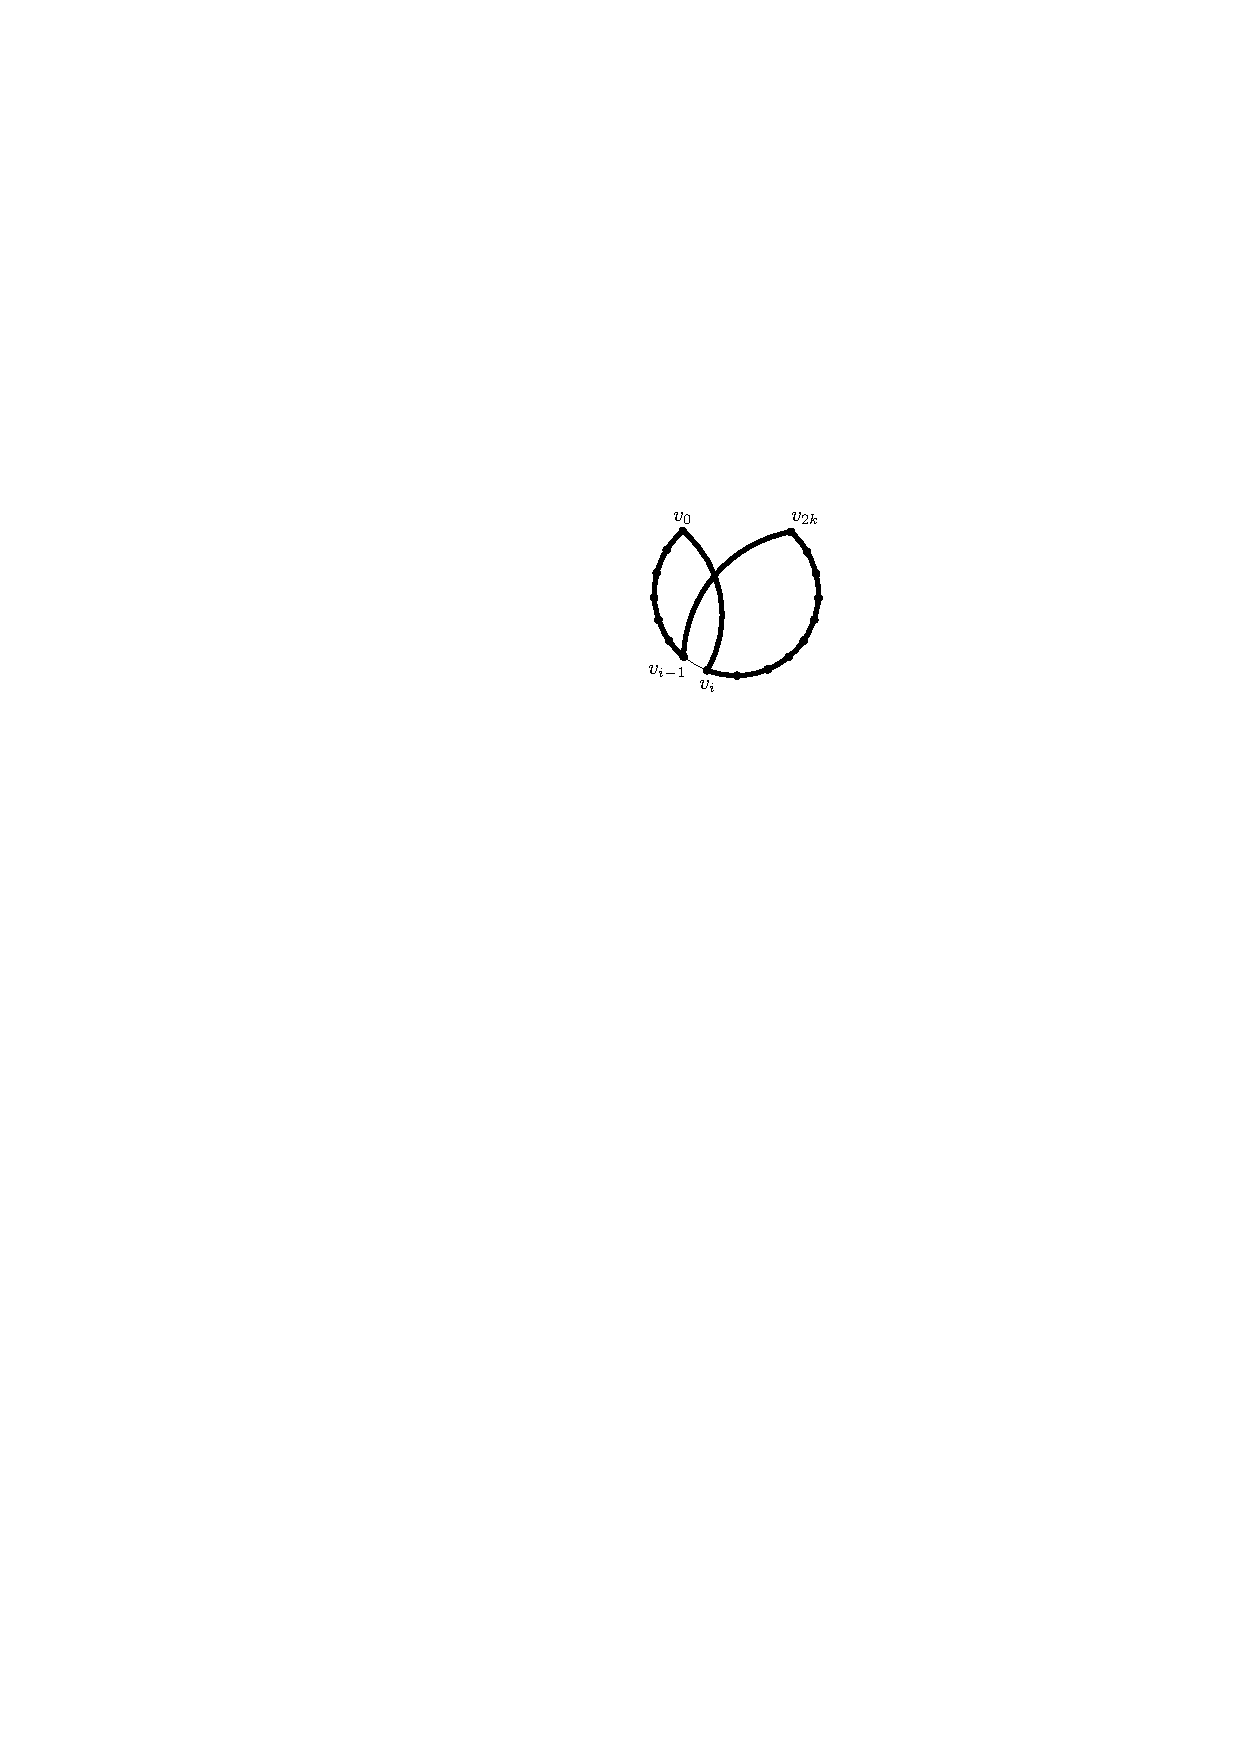
\includegraphics[width=5cm]{img/nash-williams4.pdf}
\caption{Triviální případ}
\label{dk:nw-triv}
\end{wrapfigure}

Předpokládejme že neexistuje dvojice na sousedních vrcholů $v_{i-1}v_i$, přes které by šla uzavřít kružnice (viz Obrázek \ref{dk:nw-triv}). Pak ale nutně platí, že když $v_0v_i \in E$, pak $v_{i-1}v_{2k} \not\in E$. Vrchol $v_{2k}$ má $k$ sousedů, ale nesmí mezi nimi být žádné vrcholy, jejihž pravý soused je spojen s $v_0$. Jinými slovy, $v_0$ nám vyblokuje $k$ vrcholů, do kterých nesmí vést hrana z $v_{2k}$ a ten sousedí se všemi ostatními. Tedy, když $v_0v_i \not\in E$, pak $v_{i-1}v_{2k} \in E$ (tuto vlastnost použijeme později).

\textbf{Případ (i)} $v_0$ sousedí právě s vrcholy v první polovině cesty a $v_{2k}$ právě s vrcholy v druhé polovině cesty. Pak musí existovat dvojice vrcholů $v_i,v_j$ v první polovině cesty, mezi kterými nevede hrana. Kdyby vedla hrana mezi každými dvěma vrcholy v první polovině cesty, pak by byl stupeň $v_k$ vyšší, než $k$. Protože stupeň $v_i$ je $k$, existuje $v_l$ v druhé polovině cesty tž. $v_iv_l \in E$. Pak najdu HK (viz Obrázek \ref{dk:nw-i}).

\textbf{Případ (ii)} Existuje vrchol $v_i$ takový, že $v_{i+1}v_0 \in E$, $v_iv_0 \not\in E$. Pak podle vlastnosti dokázané výše je $v_{i-1}v_{2k} \in E$. Potom $G$ obsahuje $2k$-cyklus $v_{i-1}v_{i-2}\dots v_0v_{i+1}\dots v_{2k}$ (viz Obrázek \ref{dk:nw-ii}). Přejmenujme $2k$-cyklus $C$ na $u_1u_2\dots u_{2k}$ a $u_0$ bude vrchol $G$, který v $C$ není. Potom $u_0$ nemůže sousedit se dvěma sousedními vrcholy $C$ (jinak by existovala HK) a tedy sousedí s každým druhým vrcholem $C$, řekněme s $u_1, u_3, \dots, u_{2k-1}$. Nahrazením $u_{2j}$ za $u_0$ ($\forall j$) dostaneme jiný maximální cyklus v $G$ a tedy $u_{2j}$ musí mít sousedy $u_1, u_3, \dots, u_{2k-1}$ (stejný argument jako v předchozí větě). Pak ale $u_1$ musí sousedit s $u_0, u_2, \dots, u_{2k}$ a tedy $\deg u_1 \ge k+1$, což je spor s $k$-regularitou. Tudíž je $G$ Hamiltonovský.
\qed

\begin{figure}[h]
\centering
\begin{subfigure}{7.5cm}
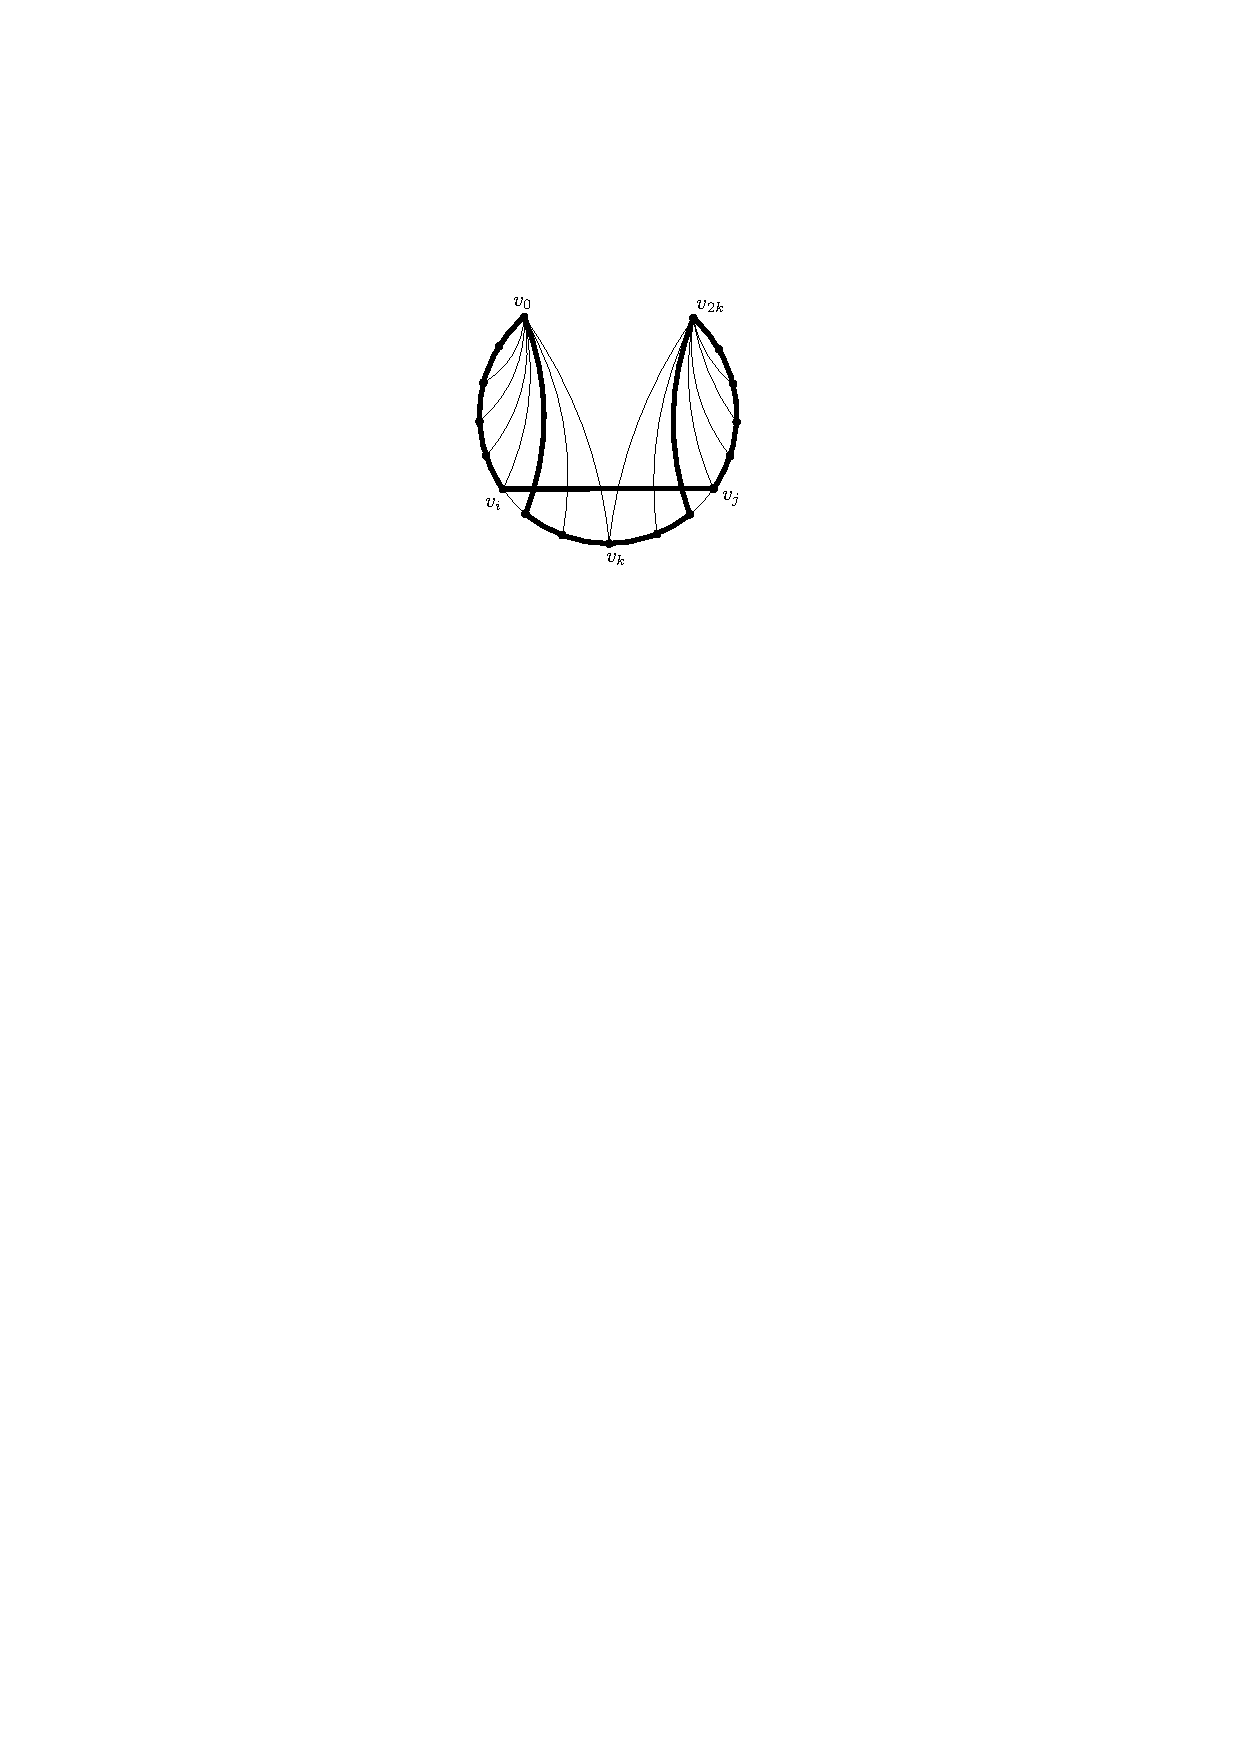
\includegraphics[width=7.5cm]{img/nash-williams2.pdf}
\caption{Případ (i)}
\label{dk:nw-i}
\end{subfigure}
\hfill
\begin{subfigure}{7.4cm}
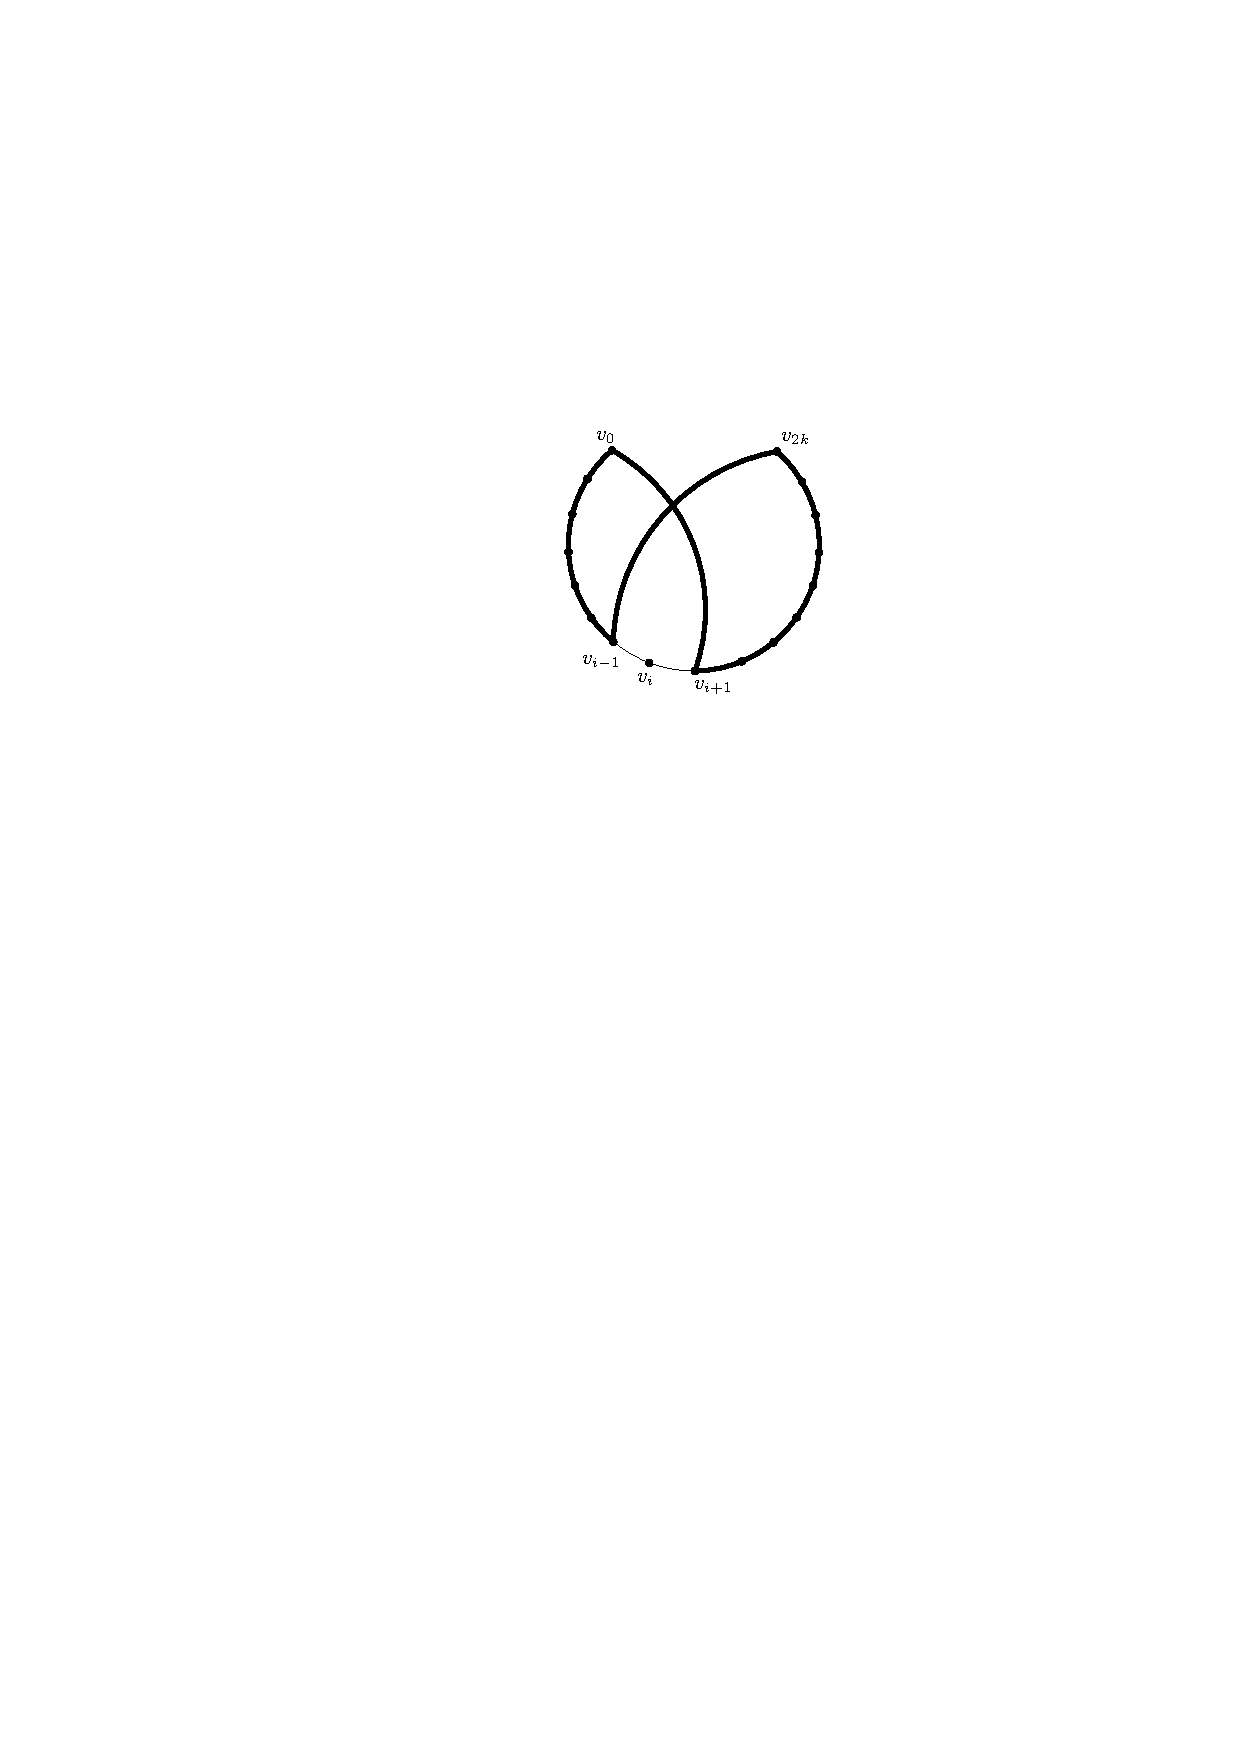
\includegraphics[width=7.5cm]{img/nash-williams3.pdf}
\caption{Případ (ii)}
\label{dk:nw-ii}
\end{subfigure}
\caption{Netriviální případy}
\end{figure}



\section{Souvislost grafů}
\df (Souvislost) Graf je hranově (vrcholově) $k$-souvislý právě tehdy, když je 
souvislý a po odebrání $k-1$ hran (vrcholů) zůstává souvislý.

\df (Souvislost orientovaných grafů) Graf $G$ je slabě souvislý, pokud je jeho 
dezorientovaný ekvivalent souvislý. Graf je silně souvislý, pokud je každá uspořádaná dvojice vrcholů $(u,v)$ spojená orientovanou cestou z $u$ do $v$.

{\it Více o silné souvislosti se nachází v sekci \ref{silna-souvislost}, včetně 
algoritmu na hledání komponent silné souvislosti.}

\vt (Ford-Fulkerson) Pro každý graf $G$ platí, že je hranově $k$-souvislý právě 
tehdy, když mezi každou dvojicí vrcholů existuje alespoň $k$ hranově 
disjunktních cest.

\vt (Menger) Pro každý graf $G$ platí, že je vrcholově $k$-souvislý právě 
tehdy, když mezi každými dvěma různými vrcholy existuje alespoň $k$ cest, které 
jsou vrcholově disjunktní (až na koncové vrcholy).

\vt (Souvislost a stupeň) Nechť $G$ má průměrný stupeň alespoň $4k$. Potom má 
$G$ $k$-souvislý podgraf.

\vt (Minimální souvislý graf) Algoritmicky najít nejmenší (co do počtu hran) 
podgraf, který je $k$-souvislý je $\NP$-těžké.

\df (Arboricita) Arboricita grafu $\A(G)$ je nejmenší počet lesů, které stačí k 
pokrytí celého grafu.

\poz (Dolní odhad na Arboricitu) Pro libovolný graf $\A(G) \geq m/(n-1)$, 
protože každá kostra má nanejvýš $n-1$ hran.

\vt (Nash-Williams) Pro graf $G=(V,E)$ platí: $\A(G) = \max_{S \subseteq V} 
\lceil m_S / (|S| -1 ) \rceil$, kde $m_S$ je počet hran grafu indukovaného na 
$S$.

\subsection{Linkovanost}

\df (Linkovanost) Graf $G$ je $k$-linkovaný, pokud pro libovolné množiny 
vrcholů $s_i, t_i, i := 1,\dots, k$ existují hranově disjunktní cesty z $s_i$ 
do $t_i$.

\pzn Linkovanost je silnější varianta souvislosti, speciálně $k$-linkovaný graf 
je určitě $k$-souvislý, naopak to neplatí; Mengerova věta totiž nezaručuje (a 
ani nemůže) propojení správných vrcholů.

\vt (Souvislost a linkovanost) Nechť $G$ je $2k$-linkovaný a obsahuje minor 
$K_{4k}$. Potom je $G$ $k$-linkovaný.

\vt (Velká souvislost a linkovanost) Nechť $G$ je $2^{4k+1}$-souvislý, potom je 
$G$ $k$-linkovaný.





\section{Speciální vlastnosti orientovaných grafů}

\label{silna-souvislost}

V orientovaných grafech se množiny hran skládají z uspořádaných dvojic vrcholů.
Oproti neorientovaným grafům rozlišujeme dva druhy souvislosti. Graf je slabě
souvislý, pokud je souvislá jeho symetrizace. Graf $G$ je silně souvislý, pokud
$\forall u,v \in V(G), u\neq v$ existuje orientovaná cesta z $u$ do $v$.
Analogicky definujeme silně souvislé komponenty (SSK) grafu $G$.

\subsection{Algoritmus pro hledání SSK}

Než popíšeme algoritmus, všimneme si nejprve několika vlastností orientovaných
grafů. Graf SSK je orientovaný acyklický graf. Proto v něm musí existovat
alespoň jedna zdrojová komponenta (do níž nevedou žádné hrany) a alespoň jedna
stoková komponenta (z níž nevedou žádné hrany). Kdybychom měli vrchol ze stokové
komponenty, mohli bychom z něj pustit DFS, který najde právě všechny vrcholy v
této SSK. Po odebrání této komponenty z grafu bychom našli novou stokovou
komponentu a pokračovali, dokud by nebyl celý graf rozdělen.

Nevíme sice, jak najít vrchol ze stokové komponenty, ale je jednoduché najít vrchol ze zdrojové komponenty -- stačí na $G$ spustit DFS (opakovaně, pokud neprošel všechny vrcholy). Vrchol, který opustíme jako poslední\footnote{Při zavedení DFS si obvykle zadefinujeme pořadí podle opouštění vrcholu, značíme $out(v)$.}, je určitě ve zdrojové komponentě. Je zjevné, že když otočíme orientaci všech hran v $G$, SSK se nezmění, pouze se ze stokových stanou zdrojové a naopak.

\lm {\it V grafu SSK $G$ vede hrana z komponenty $C_1$ do $C_2$, pak
$\max_{x\in C_1} out(x) > \max_{y\in C_2} out(y)$}

Z výše uvedeného již vyplývá jakým způsobem algoritmus pracuje: Nejprve obrátí orientaci všech hran v $G$ a najde pořadí $out(v)$ pro všechny vrcholy $G$. Poté opakovaně spouští DFS z ještě neprozkoumaných vrcholů, v pořadí od nejvyššího nalezeného $out(v)$.\footnote{Zápis algoritmu v pseudokódu je přejat z \url{http://mj.ucw.cz/vyuka/ads/25-grafy.pdf}.}

\begin{enumerate*}
\item Sestrojíme graf $G^T$ s obrácenými hranami
\item $Z \leftarrow$ prázdný zásobník
\item Pro všechny vrcholy $v$ nastavíme $komp(v) = 0$
\item Spouštíme DFS v $G^T$ opakovaně, než prozkoumáme všechny vrcholy. Kdykoliv přitom opouštíme vrchol, vložíme ho do $Z$. Vrcholy v zásobníku jsou tedy setříděné podle $out(v)$.
\item Postupně odebíráme vrcholy ze zásobníku $Z$ a pro každý vrchol $v$:
\item $\qquad$Pokud $komp(v) = 0$
\leftmargin=6cm
\indent
\item $\qquad\qquad$ Spustíme DFS($v$) v $G$, přičemž vstupujeme pouze do vrcholů s $komp(x) = 0$ a tuto hodnotu přepisujeme na $v$.
\end{enumerate*}

\dk Důkaz korektnosti algoritmu je zjevný z lemmatu a pozorování, která mu předchází. Algoritmus pouze spouští DFS a žádný vrchol neprojde vícekrát, takže se určitě zastaví. Časová i prostorová složitost jsou $\Theta(n+m)$.
\qed

Existuje i tzv. Tarjanův algoritmus pro hledání SSK, který je složitější a jeho časová i prostorová složitost je asymptoticky stejná (musí být, protože také volá DFS). Nemusí ovšem konstruovat graf s obrácenými hranami.

\subsection{Turnaje a hamiltonovské cesty}

\df (Turnaj) Turnaj je orientace úplného grafu.

\vt (O počtu Hamiltonovských cest) Existuje turnaj na $n$ vrcholech, který
obsahuje alespoň $n!/2^{n-1}$ hamiltonovských cest.

\dk Zorientujme graf nezávisle uniformě náhodně. Nechť máme permutaci $\pi$.
Jaká je pravděpodobnost, že daná permutace (tedy pořadí vrcholů) tvoří
orientovanou cestu? Máme $n-1$ hran na cestě, všechny mají permutací
předepsanou orientaci. Tedy $P(X_\pi)= 1/2^{n-1}$. Nechť $I_\pi$ je indikátor
tohoto jevu, pak $\E[I_\pi] = P(X_\pi) = 1/2^{n-1}$.

Spočítáme-li střední hodnotu počtu hamiltonovských cest, tedy součet indikátorů
přes všechny permutace, máme $n!/2^{n-1}$. Z vlastností střední hodnoty víme,
že existuje alespoň jeden graf, který má právě tolik (nebo více) hamiltonovských
cest.


\section{Algebraické vlastnosti grafů}

\subsection{Vlastní čísla grafu}

\df Vlastní čísla grafu jsou vlastní čísla matice sousednosti grafu. Množina 
vlastních čísel je {\it spektrum}, $\Sp = \{\lambda_1, \lambda_2, \dots\}$ a 
většinou se udává setříděná podle velikosti (tj. $\lambda_1$ je typicky 
největší vlastní číslo). Pro vlastní čísla platí $Ax = \lambda x$ a lze je 
vypočítat jako $\det(A - \lambda E) = 0$.

\subsection{Expandéry}

\vt (O vlastních číslech bipartitního grafu) Graf $G$ je bipartitní právě 
tehdy, když je jeho spektrum symetrické (vzhledem k nule). Pokud je navíc $G$ 
souvislý, stačí pouze $\lambda_{min} = -\lambda_{max}$.

\df Rodina expandérů $G_i$ je třída d-regulárních grafů rostoucích velikostí, 
kde každý graf má \uv{dobrou expanzí} (podle nějakého parametru).

\df (Expanze) \begin{itemize}
	\item Vrcholová expanze: $h_v(G) = \min_{S\subseteq V, |S|\leq n/2} 
	{|N(S)\setminus S| \over |S|}$.
	\item Hranová expanze: $h(G) = \min_{S\subseteq V, |S|\leq n/2} {|\delta S| 
	\over |S|}$, kde $\delta S$ značí hrany, které mají právě jeden vrchol v 
	$S$.
\end{itemize}

\poz (O hranové a vrcholové expanzi) $h_v(G) \leq h(G) \leq d \cdot h_v(G)$.

\vt (O vlastních číslech a expanzi) Pro $G$ $d$-regulární graf platí: $1/2(d - 
\lambda_2) \leq h(G) \leq \sqrt{d \cdot (d - \lambda_2)}$

\subsection{Konstrukce expandérů}

Ačkoliv například úplný graf je dobrý expandér ve smyslu, že má vysokou 
expanzi, bohužel s expanzí a velikostí roste neúnosně stupeň. Následující 
konstrukce vytváří grafy, které mají vyokou expanzi, ale konstantně malý 
stupeň.

\vt (Randomizovaná) Mějme $2n$ vrcholů. Pro $d$-regulární expandér zvolíme $d$ 
uniformě náhodných prefektních párování nad těmito vrcholy. Sjednocení těchto 
párování dává $d$-regulární graf, který je navíc dobrý expandér.

\vt (Prvočíselná) Nechť $p$ je prvočíslo a $V:=Z_p$. Definujeme $G_p=(V,E)$ s 
hranami $(x, x+1)$ a $(x,x^{-1})$ ($0^{-1}$). Pak $G_p$ je rodina dobrých 
expandérů.

\vt (Margulis) Nechť $G_m=(V,E)$ a $V=\Z_m \times \Z_M$. Definujeme hrany pro 
$4$-regulární graf jako: $(x\pm y, y)$ a $(x,y\pm x)$. Pak $G_m$ je rodina 
dobrých expandérů.

\df (Zig-Zag) Nechť $G$ je $g$-regulární graf a $H$ je $h$-regulární graf na $d$ 
vrcholech. Definujeme $G \zz H$ následujícím způsobem:
\begin{enumerate}
	\item Říkejme, že hrany z $G$ jsou {\bf\color{red}červené} a hrany z $H$ 
		jsou {\bf\color{blue}modré}.
	\item Vrcholy $G$ nahradíme grafy $H$ tak, že každému vrcholu $H$ přiřadíme 
	jednu hranu $G$. Protože $G$ je $g$-regulární a $H$ má právě $g$ vrcholů, 
	nyní každý vrchol má právě jednu hranu z $G$.
	\item Pro každou cestu tvaru 
		{\bf\color{blue}modrá}-{\bf\color{red}červená}-{\bf\color{blue}modrá} 
		vytvoříme {\bf\color{magenta}růžovou} hranu z prvního vrcholu do 
		posledního vrcholu.
	\item Odstraníme z grafu {\bf\color{blue}modré}-{\bf\color{red}červené} 
		hrany.
\end{enumerate}
Ukázka konstrukce je na obrázku \ref{zigzag-konstrukce}. Pro názornost není graf
$H$ regulární (nepodařilo se mi najít lepší příklad). Příklad je převzat z webu
\footnote{
\url{http://math.stackexchange.com/questions/454162/clearing-doubt-over-a-definition}}.

\begin{figure}
\centering
\begin{subfigure}{7.5cm}{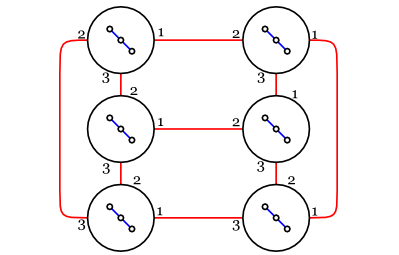
\includegraphics[width=\textwidth]{img/zigzag1.png}}\caption{Vložení 
$H$ do $G$}\end{subfigure}
\begin{subfigure}{7.5cm}{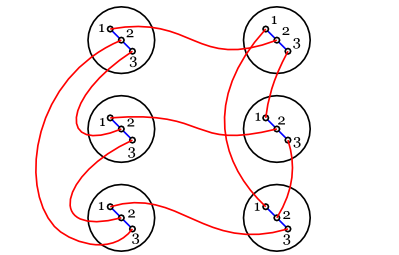
\includegraphics[width=\textwidth]{img/zigzag2.png}}\caption{Napojení 
hran $G$ na vrcholy $H$}\end{subfigure}
\begin{subfigure}{7.5cm}{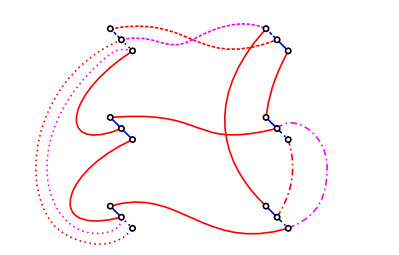
\includegraphics[width=\textwidth]{img/zigzag3.png}}\caption{Tvorba 
růžových hran}\end{subfigure}
\begin{subfigure}{7.5cm}{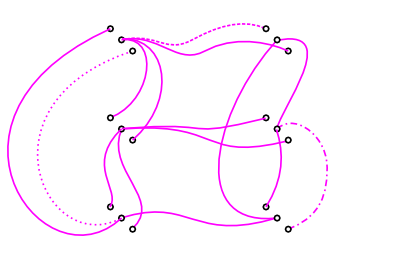
\includegraphics[width=\textwidth]{img/zigzag4.png}}\caption{Výsledek}\end{subfigure}
\caption{Příklad Zig-Zag součinu. Pro jednoduchost není $H$ regulární, na funkci
to ale nic nemění.}
\label{zigzag-konstrukce}
\end{figure}

\poz Díky této konstrukci máme graf, který zachovává velikost $G$ (dokonce ji 
zvětšuje), ale dědí stupeň po grafu $H$ (pokud stupeň byl $h$, nyní bude $h^2$ 
-- to sice není úplně dobré, ale mohlo by to být horší).

\vt (Zig-Zag) Nechť $H$ je dobrý $d$-regulární expandér, $G_1 := H^2$. Potom 
rodina grafů $G_{i+1} := G_i\zz H$ je dobrý expandér.


\pagebreak
\section{Teorie párování}
\subsection{Párování na množinách}

\df Systém různých reprezentantů (SRR) {\it množinového systému $(X,S)$ je
prostá funkce $f:S\rightarrow X$ tž. $\forall A \in S: f(A) \in A$.}

\vt (spočetná Hallova) {\it Buď $(X,S)$ množinový systém obsahující spočetně mnoho konečných množin. Pak $(X,S)$ má SRR právě tehdy, když pro libovolný podsystém $T \subseteq S$ s konečně mnoha podmnožinami platí $|\bigcup T| \ge |T|$} (Hallova podmínka)

\dk {\it (v sekci \ref{nekonecna-kombinatorika:hall})}

\subsection{Párování v grafech}

\df Párování je množina hran $M$ taková, že žádné dvě hrany nesdílí společný
vrchol. {\it Perfektní párování} je takové párování, které je incidentní se
všemi vrcholy grafu.

\tv Maximální párování na bipartitním grafu lze nalézt pomocí toků v sítích v
čase $\O(|E| \cdot |M|)$.

\vt Maximální párování v obecném grafu lze nalézt pomocí Edmondsova algoritmu v
čase $\O(|V|^2|E|)$.

\df Vylepšující cesta je cesta, která začíná i končí hranou z $G$, která není v
párování $M$, a na cestě se střídají hrany z $M$ a $E\setminus M$.

\vt (Berge) Párování je maximální právě tehdy, pokud neexistuje vylepšující
cesta.

\alg (Edmondsův květinkový) Algoritmus v každá iterace nalezne zlepšující cestu
a zvětší párování, pokud větší existuje. Díky předchozí větě pokud algoritmus
nenalezne zlepšující cestu, víme, že vydá maximální párování. Zlepšující cesta
se hledá následujícím způsobem:

\begin{enumerate}
	\item Najdi nespárované vrcholy a prohlaš je za kořeny stromů v lese.
	\item Pro každý vrchol přidej do stromu jeho sousedy tak, že na 1. patře je
	pouze kořen, všechny hrany z kořene jsou z $E \setminus M$ a všechny cesty
	od kořene k listům jsou střídavé. Po každém přidání zkontroluj:
	\begin{enumerate}
		\item Vytvořil se lichý cyklus? Pokud ano, kontrahuj ho a pokračuj.
		\item Vede z aktuálního vrcholu hrana do jiného stromu taková, že lze
		vytvořit vylepšující cestu? Pokud ano, vydej tuto cestu.
	\end{enumerate}
	\item Pokud nelze přidat další vrchol, vydej dosavadní párování jako
	maximální.
\end{enumerate}

Algoritmus tedy buduje stromy, pro které cesta kořen-kořen je zlepšující. Liché
cykly se kontrahují, protože bez nich je těžké poznat, zda se nalezla zlepšující
cesta (viz obrázek \ref{blossoms}, kde modrá hrana vytvoří květinku a až po
jejím přidání je možné použít červenou hranu na vylepšující cestu; kotrakce
zjednoduší uvažování cyklů).

Kontrakce nerobijí existenci střídavých cest, protože každá střídavá cesta musí
vést přes stonek, tedy od propojení směrem ke kořeni (jenom v kořeni jsou
vrcholy, kterými lze střídavou cestu ukončit) a každá střídavá cesta si může
vybrat, zda první krok v květince udělá po spárované nebo nespárované hraně.

Vylepšujících cest je najevýš $|E| = m$ po celou dobu běhu algoritmu, jedno
prohledávání spotřebuje nanejvýš $n^2$ času (práce na každém vrcholu může být až
$n$, protože je potřeba potenciálně prohledat hodně sousedů). Celkový běh
algoritmu je tedy $\O(n^2m)$. \qed

\begin{figure}[h!]
	\centering
	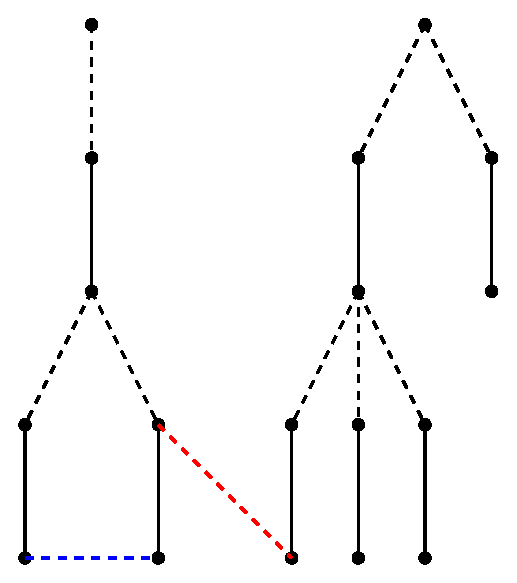
\includegraphics{img/blossoms.eps}
	\caption{Tvorba cyklů a vylepšujících cest v květinkovém algoritmu}
	\label{blossoms}
\end{figure}

\subsection{Otázka velikosti maximálního párování}

\vt (König) Velikost maximálního párování bipartitního grafu odpovídá velikosti
minimálního vrcholového pokrytí.

\vt (Hall) Bipartitní graf $G$ má perfektní párování právě tehdy, když pro každé
$X \subseteq V$ je počet izolovaných vrcholů $G \setminus X$ nanejvýš $X$.

\vt (Tutte) Graf $G$ má perfektní párování právě tehdy, když pro každé $X
\subseteq V$ je počet lichých komponent $G \setminus X$ nanejvýš $|X|$.

\vt (Petersen) Každý 3-regulární graf bez mostů má perfektní párování.

\dk Ukážeme, že každá $X$ splňuje Tutteho podmínku. Označme $q(G \setminus X)$
počet lichých komponent $G \setminus X$. Nechť máme libovolnou $X$ a nějakou
lichou komponentu $C$ (pokud taková neexistuje, podmínka je splněna
automaticky).  Komponenta $C$ má lichý počet vrcholů, ale sudý součet stupňů
(jako každý graf), do grafu ale přispívá celkově lichým součtem stupňů (má lichý
počet vrcholů, každý 3 hrany) -- počet hran spojující $C$ se zbytkem grafu je
tedy lichý, a navíc alespoň $3$, protože jedna hrana by tvořila most. Tedy počet
hran vedoucích z $X$ je alespoň $3q(G \setminus X)$, ale taktéž nanejvýš $3|X|$,
což je maximální počet hran v $S$ z $3$-regularity. Máme tedy $3q(G \setminus X)
\leq\delta X \leq 3|X|$, což po vykrácení $3$ dává Tutteho podmínku a věta je
dokázána. \qed


\subsection{Matching polytope}

Párování stálo u základů polyedrální kombinatoriky, a tak je vhodné zmínit
polytopy, které problém řeší:

\df Označme $\delta(v)$ množinu hran incidentních s vrcholem $v$, $x(e)$ jako
proměnnou pro hranu $e$ a $x(\delta(v)) := \sum_{e \in\delta(v)} x(e)$.

\tv Pro bipartitní graf je Matching polytope následující:
\begin{align}
	x(\delta(v)) \leq 1  & \quad  \forall v \in V \\
	x(e) \geq 0 & \quad \forall e  \in E
\end{align}

Takový polytop (překvapivě) má vždy celočíselné optimální řešení, ale může se
stát, že získáme neceločíselné a přesto optimální (například čtyřcyklus
ohodnocený 1/4). O to horší by byl výsledek tohoto polytopu u nebipartitních
grafů, protože na lichém cyklu získáme lepší neceločíselné, než nejlepší
celočíselné řešení; viz obrázek \ref{matching-polytope}.

Ukazuje se však, že protože matice incidence pro bipartitní graf je totálně
unimodulární, všechna řešení nalezená simplexovým algoritmem jsou celočíselná.

\df Matice $A$ je totálně unimodulární, pokud determinant každé její čtvercové
podmatice je $-1, 0$ nebo $1$.

\df Pokud je $Ax \leq b$ lineární program a $A$ je totálně unimodulární, jsou
všechny vrcholy daného polyedru celočíselné.

\begin{figure}[h!]
	\centering
	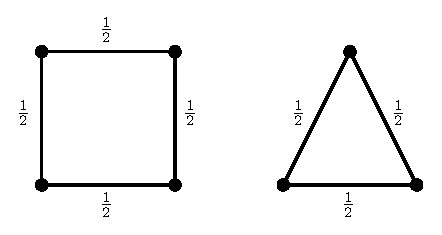
\includegraphics{img/matching-polytope.eps}
	\caption{Ukázka nevhodných neceločíselných řešení}
	\label{matching-polytope}
\end{figure}

\tv Pro libovolný graf je Matching polytope pro perfektní párování následující:
\begin{align}
	x(\delta(v)) \leq 1  & \quad  \forall v \in V \\
	x(e) \geq 0 & \quad \forall e  \in E \\
	x(\delta(U)) \geq 1 & \quad \forall U \subseteq V, |U| \geq 3 \text{ liché
velikosti}
\end{align}

\tv Pro libovolný graf je Matching polytope pro maximální párování následující:
\begin{align}
	x(\delta(v)) \leq 1  & \quad  \forall v \in V \\
	x(e) \geq 0 & \quad \forall e  \in E \\
	x(E[U]) \leq {|U|-1 \over 2} & \quad \forall U \subseteq V, |U| \text{ liché
velikosti}
\end{align}


\section{Ramseyova teorie}
Ramseyova teorie zkoumá především výskyt zajímavých struktur na velmi velkých grafech. Ramseyových vět existuje hned několik, začneme ovšem jinou extremální větou a to Turánovou. Hlavními výsledky v Ramseyově teorii jsou Hales-Jewett a Van der Waerdenova věta.

\subsection{Turánova věta}

\df Turánův graf $T(n,r)$ {\it je graf na $n$ vrcholech, které byly rozděleny do $r$ skupin, jejichž velikost se liší nejvýš o 1. Hrana vede mezi každými dvěma vrcholy, které nejsou ve stejné skupině.}

Turánovy grafy jsou pokus o konstrukci hranově extremálních grafů neobsahujících podgraf $K_{r+1}$. Turánova věta nám pak říká, že turánovy grafy mají skutečně maximální možný počet hran.

\vt (Turánova, verze 1) {\it Ze všech grafů na $n$ vrcholech, které neobsahují $K_{r+1}$ jako podgraf má $T(n,r)$ nejvyšší počet hran.}

\vt (Turánova, verze 2) {\it Nechť $G$ je graf na $n$ vrcholech neobsahující $K_{r+1}$ jako podgraf. Pak počet hran $G$ je nejvýš ${r-1\over r}\cdot{n^2\over 2} = \left(1-{1\over r}\right)\cdot{n^2\over 2}$.}

\dk (Turánovy věty): Předpokládejme, že $G$ je graf neobsahující $K_{r+1}$ s
maximálním počtem hran. V první části důkazu ukážeme, že $G$ musí být úplný
$r$-partitní graf, v druhé části že se velikost jednotlivých partit může lišit
nejvýš o 1.

\textbf{Část 1.} Graf $G$ neobsahuje trojici vrcholů $u$, $v$, $w$ tž. hrana
vede pouze mezi $u$ a $v$. To dokážeme tak, že buď smažeme $w$ a zkopírujeme
$u$, nebo smažeme $u$ a $v$ a zkopírujeme dvakrát $w$, čímž dostaneme graf s
více hranami. Z toho plyne, že můžeme vrcholy $G$ rozdělit do tříd ekvivalence
na základě nesousednosti (dva vrcholy jsou ve stejné třídě, když mezi nimi
nevede hrana). Třídy ekvivalence tvoří partity a $G$ je tedy úplný
multipartitní graf. Čím více partit, tím více hran, takže $G$ je úplný
$r$-partitní graf.

\begin{figure}[h]
\centering
\begin{subfigure}{8cm}
\begin{subfigure}{3cm}
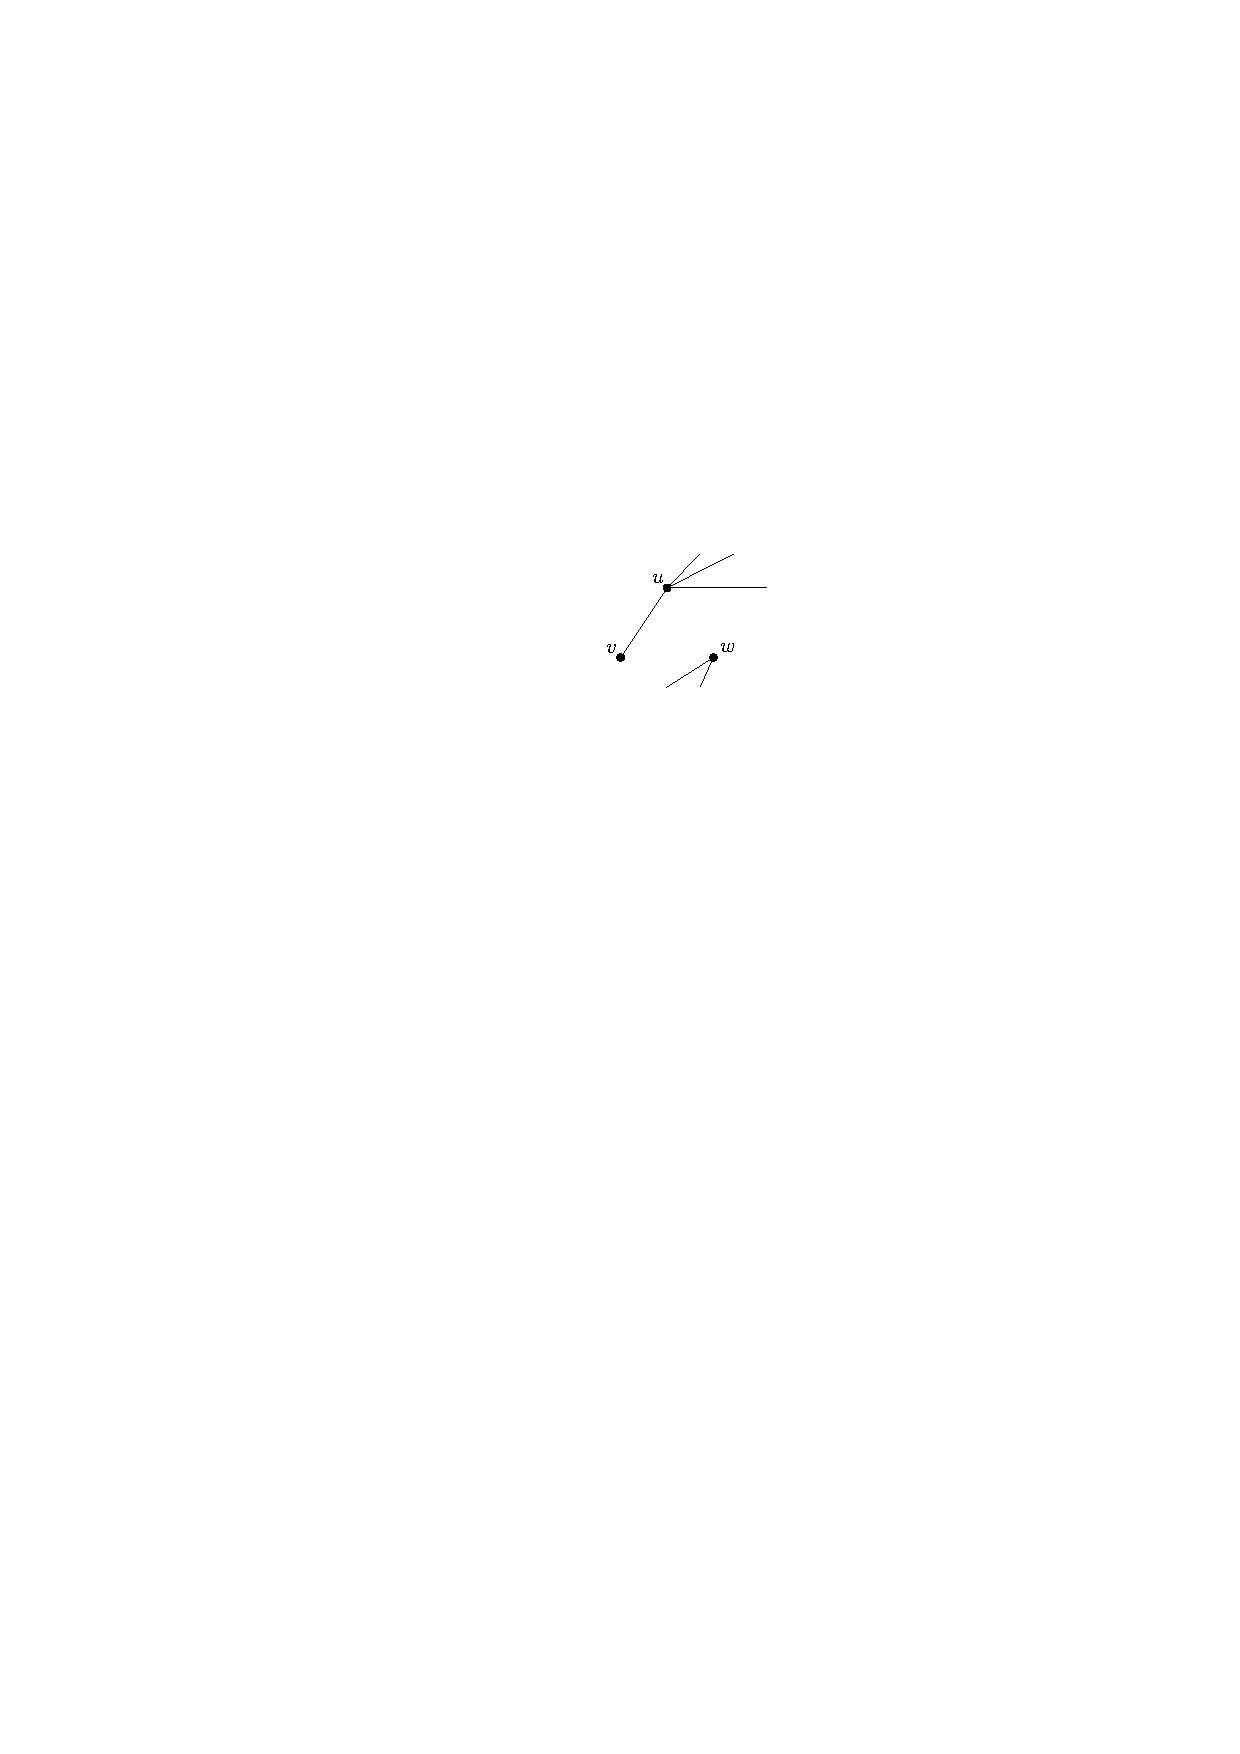
\includegraphics[width=3cm]{img/turan1.pdf}
\end{subfigure}
\hspace{0.5cm}$\Rightarrow$\hspace{0.5cm}
\begin{subfigure}{3cm}
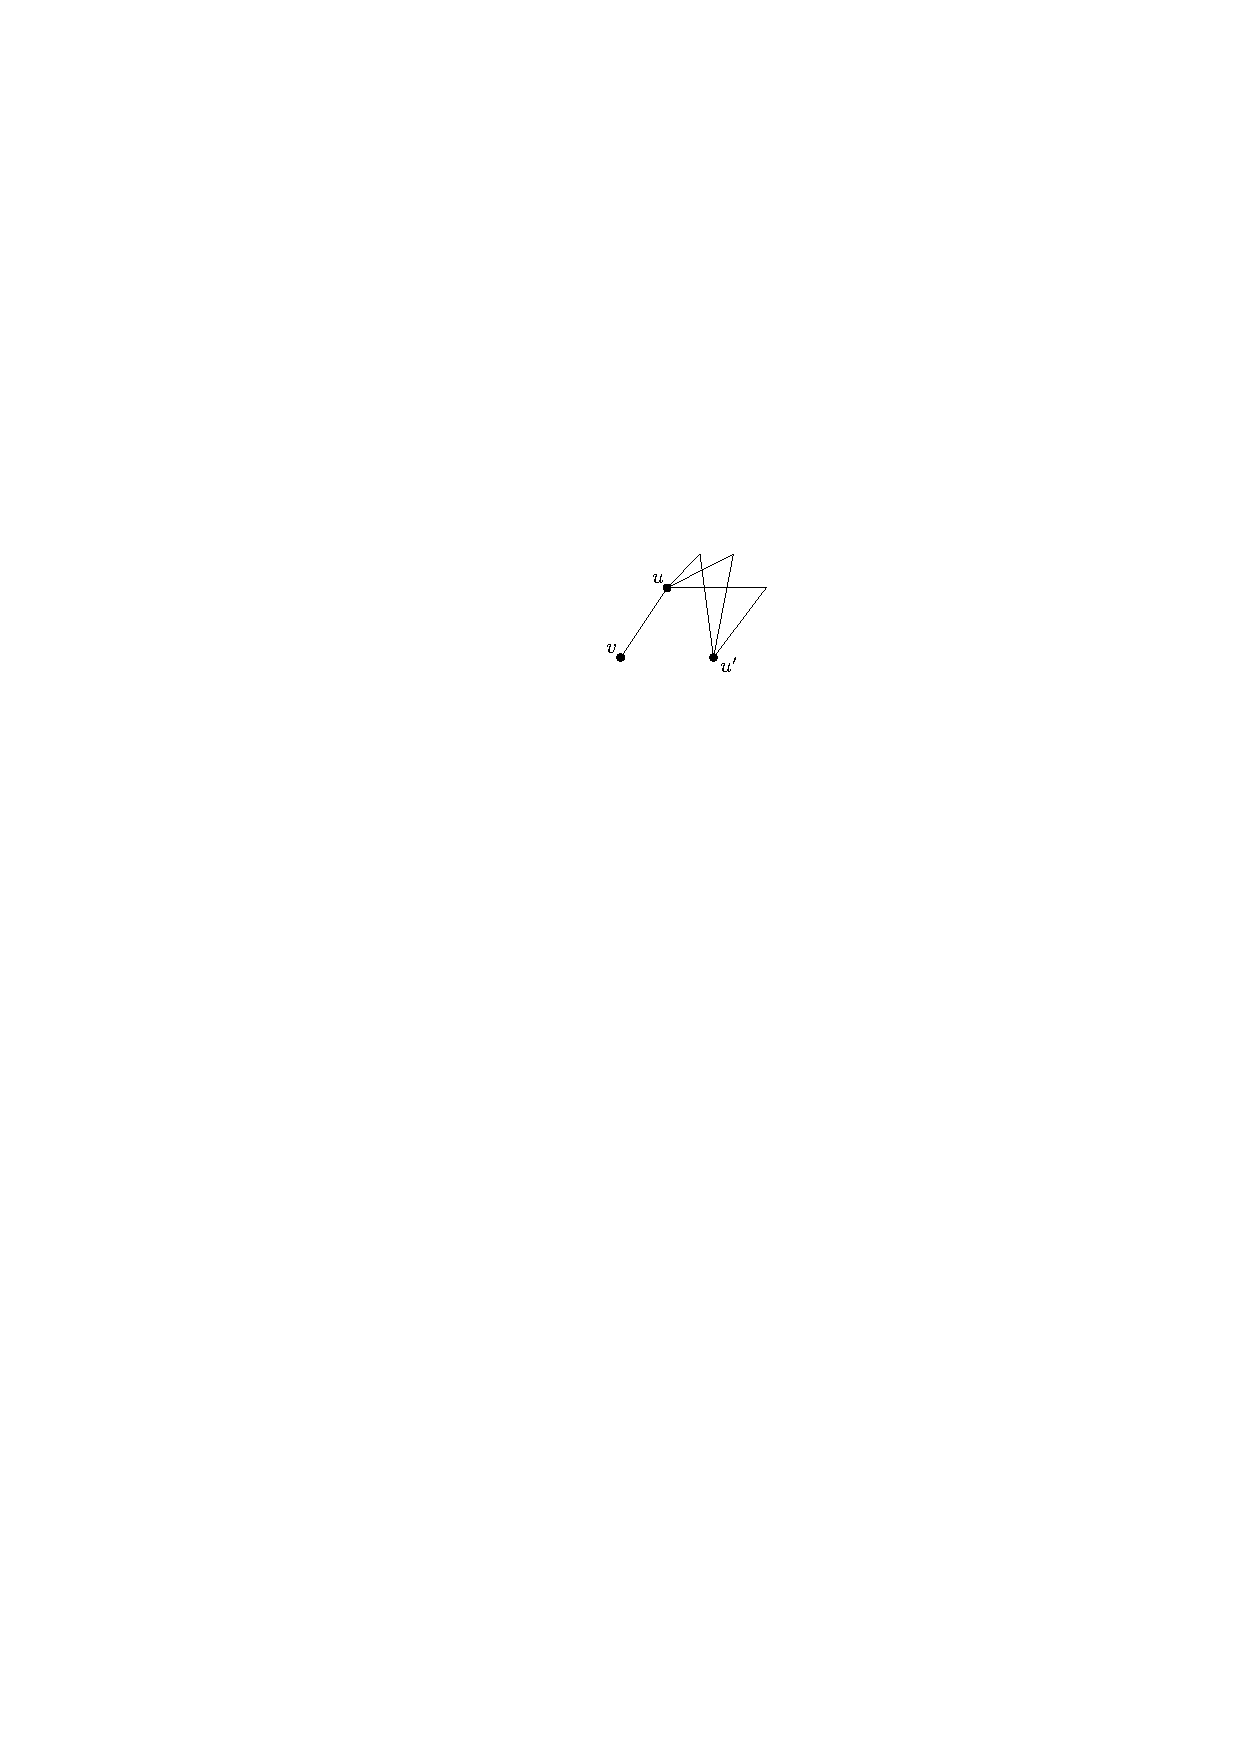
\includegraphics[width=3cm]{img/turan2.pdf}
\end{subfigure}
\caption{$d(w) < d(u)$}
\end{subfigure}
\hfill
\begin{subfigure}{8cm}
\begin{subfigure}{3cm}
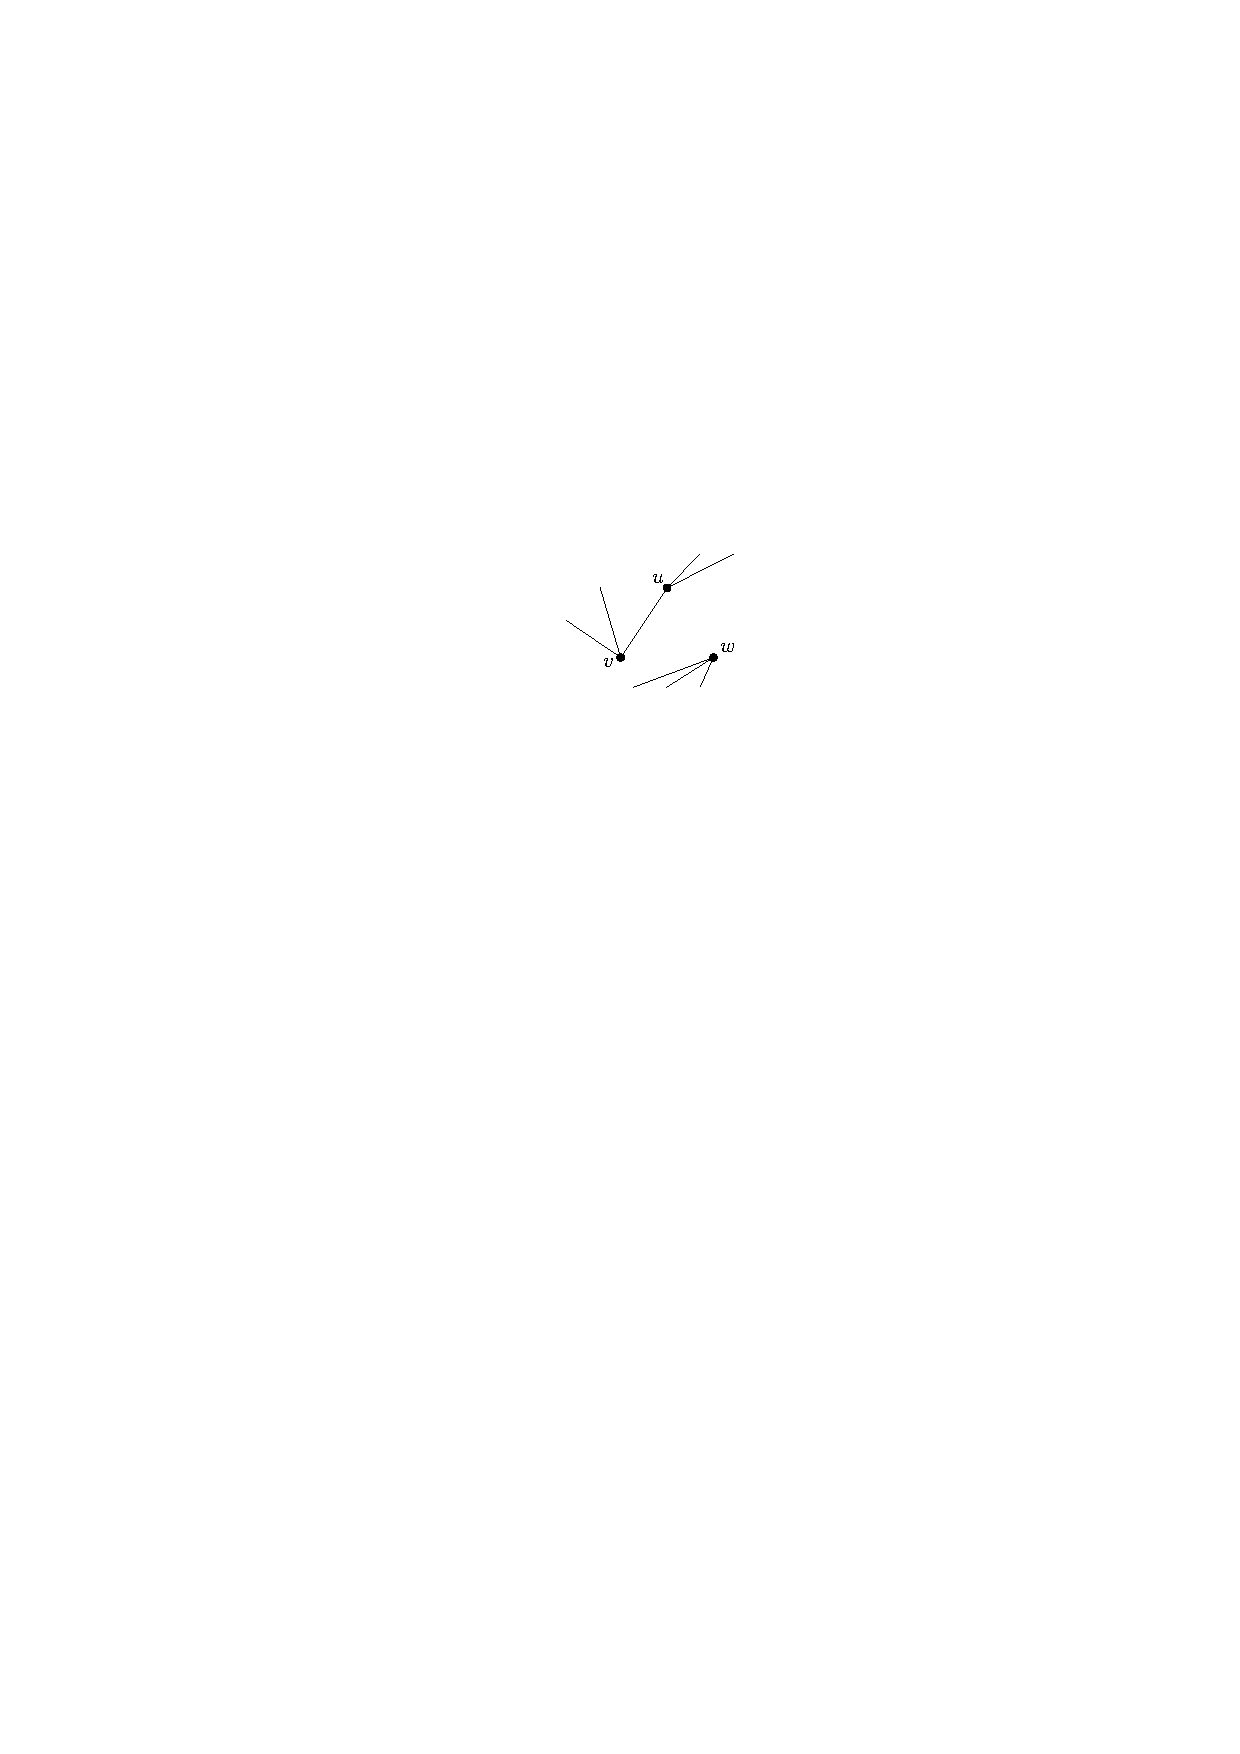
\includegraphics[width=3cm]{img/turan3.pdf}
\end{subfigure}
\hspace{0.5cm}$\Rightarrow$\hspace{0.5cm}
\begin{subfigure}{3cm}
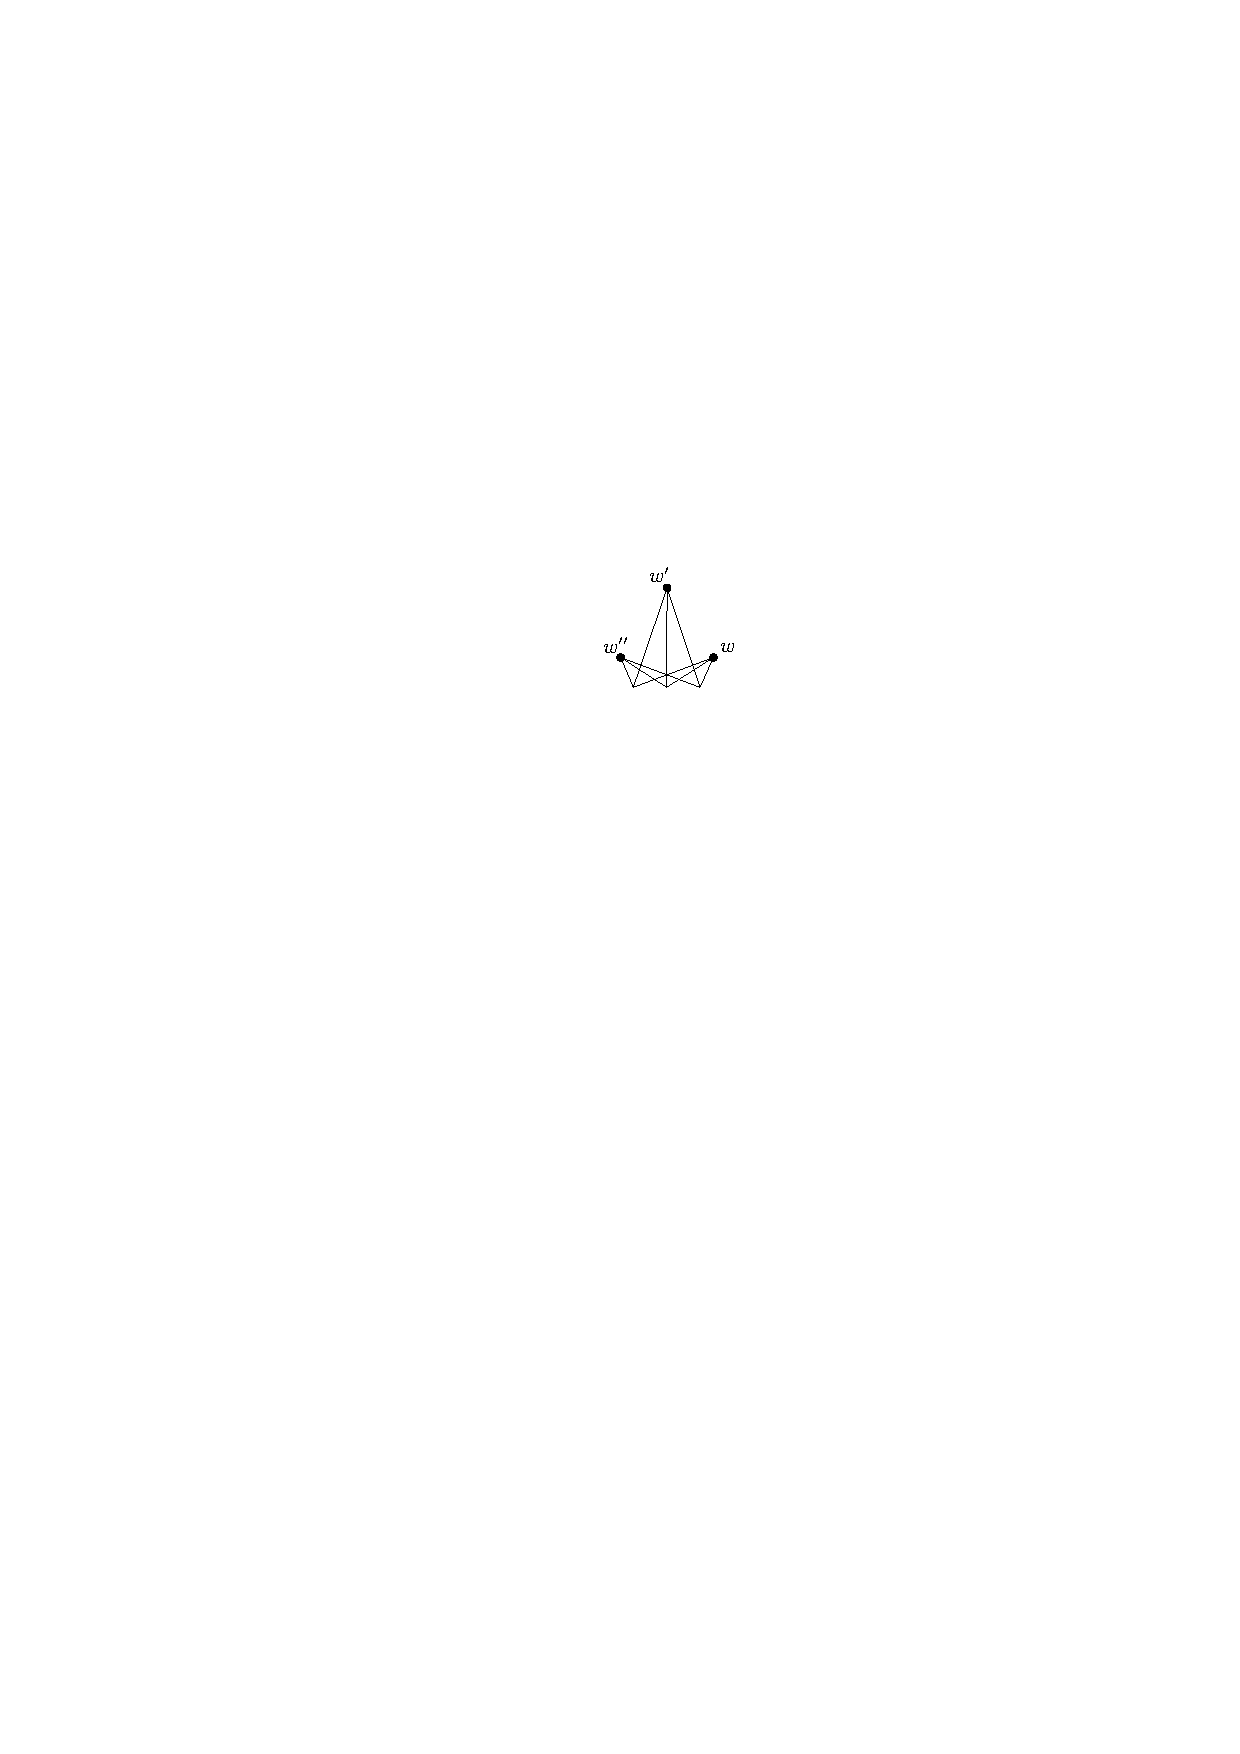
\includegraphics[width=3cm]{img/turan4.pdf}
\end{subfigure}
\caption{$d(w) \ge d(u)$ a $d(w) \ge d(v)$}
\end{subfigure}
\caption{Důkaz Turánovy věty, část 1.}
\end{figure}

\textbf{Část 2.} Mějme partity $A$ a $B$ tž. $|A| > |B| + 1$. Pak přesunem
vrcholu z $A$ do $B$ ztratíme $|B|$ hran, ale získáme $|A|-1$ hran a tedy
zvýšíme počet hran v $G$ alespoň o 1. Tedy, počet hran v $r$-partitním grafu je
maximální, když se velikosti partit liší nejvýše o 1. 
\qed

\subsection{Ramseyovy věty}

\vt (Ramsey) {\it Pro každé $k \in \N$ existuje $n \in \N$ tž. každý graf na alespoň $n$ vrcholech obsahuje $K_k$ nebo indukovaný $\overline{K_k}$ jako podgraf.\footnote{Nejmenší takové $n$ pro dané $k$ nazýváme Ramseyovo číslo a značíme $R(k)$.}\footnote{Můžeme se setkat i s verzí, kdy určujeme velikost kliky a velikost nezávislé množiny zvlášť. Pak značíme Ramseyovo číslo $R(k,l)$.}}

\vt (Ramsey, vícebarevná) {\it Pro každé $t$ a $k$ existuje $N$ takové, že pro každou funkci $c: {[n]\choose 2} \rightarrow [t], n\geq N$ existuje množina $A \in {[n]\choose k}$, pro níž je funkce $c$ na $A\choose 2$ konstantní.} Jinými slovy, existuje dostatečně velké $N$ takové, že každý úplný graf alespoň na $N$ vrcholech obarvený $t$ barvami obsahuje jednobarevnou kliku velikosti $k$.

\vt (Ramsey, nekonečná) {\it Pro každé $t$ a každou funkci $c: {\N\choose 2} \rightarrow [t]$ existuje nekonečná množina $A\subseteq \N$, pro níž je funkce $c$ na $A\choose 2$ konstantní.} Neboli, v každém nekonečném úplném grafu obarveném $t$ barvami existuje nekonečně velká monochromatická klika.

\dk Sestrojíme si nekonečnou posloupnost nekonečných množin $A_1, A_2, \dots$ Začneme s $A_1 = \N$. Z $A_i$ zkonstruujeme $A_{i+1}$ tak, že si vybereme nejmenší prvek\footnote{Mohl by být libovolný, ale takhle se elegantně vyhneme problému s axiomem výběru.} $v_i \in A_i$ a rozdělíme vrcholy $A_i \setminus \{v_i\}$ na třídy ekvivalence $B_i^1, \dots, B_i^t$ podle toho, jakou barvu má hrana, která je spojuje s $v_i$. Podle nekonečného principu holubníku je alespoň jedna z $B_i^j$ nekonečná. Položme $b_i = j$ a $A_{i+1} = B_i^j$ a pokračujme dalším krokem (do nekonečna).

Všimněme si, že v posloupnosti vybraných vrcholů $(v_i)$ platí $\forall i < j$ má hrana $v_iv_j$ barvu $b_i$ (tedy záleží pouze na vrcholu s nižším pořadovým číslem). V nekonečné posloupnosti $b_1,b_2,\dots$ se musí některá z $t$ barev opakovat nekonečněkrát -- odpovídající vrcholy pak tvoří jednobarevný nekonečný úplný graf.
\qed

Konečná verze se dokazuje obdobně, ale musíme pečlivěji upočítat potřebnou velikost počáteční množiny.

\subsection{Hales-Jewett}

Zjednodušeně řečeno, Hales-Jewettova věta praví, že když dostanu od protivníka délku hrany krychle $a$ a počet barev $r$, dokážu najít dostatečně velkou dimenzi $N$, aby každé obarvení $N$-dimenzionální krychle o hraně $a$ pomocí $r$ barev obsahovalo jednobarevnou piškvorku délky $a$. Dále budeme značit $A = \{1, \dots, a\}$.

\vt (Hales-Jewett) {\it Pro každé $a$ (délka hrany krychle) a $r$ (počet barev) existuje $N = HJ(r,a)$ tž. obarvíme-li body krychle $A^N$ pomocí $r$ barev, vždy existuje jednobarevná kombinatorická přímka.}

\tv (o vnořené konzistentní krychli) {\it Existuje $N$ takové, že pro každé obarvení $\chi: A^N \rightarrow {1,\dots, r}$ existuje podkrychle $\alpha[A^n] \subset A^N$ obarvená konzistentně.} Konzistentně obarvená krychle znamená, že barvy na vnější slupce (bodech, jejichž nějaká souřadnice je 0) jsou kopiemi barev sousedních vrcholů o jednu vrstvu hlouběji.

\dk \textbf{(Idea)} Zafixujeme si $r$ a důkaz provedeme indukcí podle $a$. Pro $a=1$ je situace triviální. Pro větší $a$ použijeme pomocné tvrzení o vnořené konzistentní krychli a najdeme krychli $A^n$. Z té sloupneme vnější slupku, v krychli s o jedna kratší hranou nalezneme piškvorku (z indukčního předpokladu) a po doplnění slupky dostaneme piškvorku v $A^n$ (protože krychle je konzistentní). Piškvorka v $A^n$ je i piškvorkou v $A^N$ (jedná se o vnoření), čímž je indukční krok hotový.
\qed

Důkaz pomocného tvrzení je technický, takže jen uvedeme konstrukci $N$, abychom měli představu o jeho velikosti. Zadefinujeme $N = N_1 + \dots + N_n$, kde:

$$N_1 = r^{a^n},\qquad N_i = r^{a^{\left(n+\sum_{j=1}^{i-1} N_j\right)}}$$

\subsection{Van der Waerden}

\vt (Van der Waerden) {\it Pro každé $r, k \in \Z^+$ existuje $N$ takové, že v každém obarvení posloupnosti ${1, 2, \dots, N}$ $r$ barvami najdeme jednobarevnou aritmetickou posloupnost délky alespoň $k$.}

V praxi je takové $N$ obludně velké, nejlepší známý horní odhad tvrdí $W(r,k) \le 2^{2^{r^{2^{2^{k+9}}}}}$.

\dk Použijeme Hales-Jewetta a najdeme $N = HJ(r,k)$. Každé číslo $a \in \{0, 1, \dots, t^N-1\}$ můžeme zapsat v soustavě o základu $t$ jako $(a_0,a_1,\dots,a_{N-1})$, kde $a = a_0 + a_1t + \dots + a_{N-1}t^{N-1}$. Tím jsme získali bijekci mezi čísly od 0 do $t^N-1$ a vrcholy $N$-dimenzionální krychle o hraně $k$. Z Hales-Jewetta víme, že v krychli existuje kombinatorická přímka délky $k$. Kombinatorická přímka odpovídá aritmetické posloupnosti -- jedna její souřadnice nabývá hodnot od 0 do $N-1$ a všechny ostatní zůstávají konstantní.
\qed



\section{Nekonečná kombinatorika}

\vt (Cantor-Bernstein) {\it Nechť $A$ a $B$ jsou dvě množiny, pro které existují prostá zobrazení $f: A \rightarrow B$ a $g: B \rightarrow A$. Potom existuje bijekce $h: A \rightarrow B$.

\dk Sestrojíme bipartitní graf a ukážeme, že ve všech jeho komponentách existuje párování. Hezky popsáno v \texttt{http://mj.ucw.cz/papers/kg1.pdf}

\subsection{Königovo nekonečné lemma}

\lm (Königovo nekonečné lemma) Nechť $V_0,V_1,\dots$ je nekonečná posloupnost disjunktních neprázdných konečných množin a $G$ je graf jejich sjednocení. Předpokládejme, že každý vrchol $v \in V_n$ má souseda $f(v) \in V_{n-1}$. Potom $G$ obsahuje nekonečnou cestu $v_0v_1\dots$, kde $\forall n\in \N: v_n\in V_n$.

\medskip\noindent {\bf Důsledek} V každém zakořeněném stromu, který má nekonečně mnoho vrcholů, ale pouze konečné stupně, existuje nekonečná cesta začínající v kořeni.

\dk Vezmeme všechny konečné cesty končící ve $V_0$. Těch je nekonečně, takže z principu holubníku existuje $v_0\in V_0$ tž. jím prochází nekonečně mnoho konečných cest. Některým z jeho sousedů $v_1\in V_1$ prochází také nekonečně mnoho konečných cest. Tímto argumentem můžeme pokračovat neomezeně a vygenerovat tak hledanou nekonečnou cestu $v_0v_1\dots$
\qed

Königovo lemma lze využít v důkazu věty o kompaktnosti výrokové logiky.\footnote{\it Spočetná množina formulí $\Psi$ je splnitelná právě tehdy, když je splnitelná každá její konečná podmnožina.}

\subsection{Věta o barevnosti nekonečných grafů}

\vt (Bruijn \& Erdös, 1951) {\it Nechť $G$ je graf a $k\in \N$. Pokud je každý konečný podgraf $G$ obarvitelný nejvýše $k$ barvami, pak je nejvýše $k$ barvami obarvitelný i $G$.}

\dk Mějme očíslování vrcholů $G$ $v_0, v_1, \dots$ Definujeme $G_n = G[v_0,\dots, v_n]$. Množinu všech $k$-obarvení grafu $G_n$ označíme $C_n$. Vytvoříme graf, jehož vrcholy tvoří jednotlivá obarvení $\bigcup_{n\in\N} C_n$ a hrany $cc'$ tž. $c\in C_n$ a $c'\in C_{n-1}$ (tedy hrany vedou mezi obarvením grafu s $n-1$ vrcholy, do všech rozšíření tohoto obarvení na graf s $n$ vrcholy). V tomto grafu dle Königova nekonečného lemma najdeme nekonečnou cestu $c_0c_1\dots$ tž. $\forall n\in\N: c_n \in C_n$. Potom $c := \bigcup_{n\in\N}c_n$ je obarvení grafu $G$ $k$ barvami.
\qed

\subsection{Hallova věta}
\label{nekonecna-kombinatorika:hall}

\df Systém různých reprezentantů (SRR) {\it množinového systému $(X,S)$ je prostá funkce $f:S\rightarrow X$ tž. $\forall A \in S: f(A) \in A$.}

\vt (spočetná Hallova) {\it Buď $(X,S)$ množinový systém obsahující spočetně mnoho konečných množin. Pak $(X,S)$ má SRR právě tehdy, když pro libovolný podsystém $T \subseteq S$ s konečně mnoha podmnožinami platí $|\bigcup T| \ge |T|$} (Hallova podmínka)

\dk Technický. Pro každý prvek $x \in X$ zavedeme výrokovou proměnnou $a_x$ a nadefinujeme si výrokové formule tak, aby vyjadřovaly podmínky, že každá množina má reprezentanta a dvě různé množiny nemají stejného reprezentanta. Potom použijeme větu o kompaktnosti výrokové logiky.



\section{Strukturální vlastnosti množinových systémů}
\subsection{Extrémální vlastnosti}

\df Slunečnice (někdy také $\Delta$-systém) s $k$ lístky a jádrem $Y$ je systém 
množin $S_1, \dots, S_k$ takových, že $\forall i\neq j: S_i \cap S_j = Y$ a 
navíc $S_i \setminus Y \neq \emptyset$.

\vt (Slunečnicové lemma) Nechť $\F$ je množinový systém s množinami velikosti 
$s$.  Pokud $|\F| > s!  (k-1)^s$, potom $\F$ obsahuje slunečnici s $k$ lístky.

\dk Indukcí podle $s$. Pro $s=1$ máme alespoň $k-1$ jednoprvkových množin, a 
všechny tvoří slunečnici s malými lístky a prázdným jádrem. Dále nechť $s\geq 
2$: $\A := \{A_1, \dots, A_t\}$ označme maximální systém po dvou disjunktn9ch 
množin z $\F$. Pokud $t \geq k$, tvoří slunečnici s prázným jádrem a máme 
hotovo. Jinak vezměme $B := \bigcup_i A_i$; pro tu platí $|B| \leq s\cdot 
(k-1)$ a nějaký prvek, říkejme mu $x$, se vyskytuje v hodně množinách, 
konkrétně z holubníkového principu:
\begin{align*}
	{|\F| \over |B|} > (s-1)!(k-1)^{s-1}
\end{align*}
Takových množin je dokonce tolik, že samy o sobě splňují nutnou podmínku pro 
slunečnici velikosti $k$ v množinách o $1$ menších. Aplikujeme tedy indukci na 
systém $\F_x := \{S - x: S \in \F, x \in S\}$ a do výsledné slunečnice prvek 
$x$ vrátíme.

\vt (Slunečnicová spekulace) Ve slunečnicovém lemmatu stačí dokonce $|\F| \geq 
c_k^s$, kde $c_k$ je nějaká konstanta.

\pzn Ačkoliv Slunečnicové lemma zahřeje zevnitř, jeho aplikace se příliš 
nezmiňují. Zde je jedna:

Je otevřeným problémem, zda existuje algoritmus na násobení matic v čase 
$n^{2+\epsilon}$ pro každé $\epsilon$. Postup Coppersmitha a Winograda nabízí 
jednu z možností, jak takový algoritmus sestrojit; speciálně potřebují získat 
speciální Abelovskou grupu splňující hromádku požadavků; lze ukázat, že 
existence takové grupy je ve sporu se Slunečnicovou spekulací. To ale 
neznamená, že i kdyby Slunečnicová spekulace byla pravdivá, že neexistuje 
rychlý algoritmus na násobení matic, jsou další postupy, jak toho dosáhnout 
(speciálně Cohn-Umans).


\vt (Erdös-Ko-Rado) Nechť $n \geq 2k$, potom každý průsečný systém 
$k$-prvkových podmnožin $n$-prvkové množiny má nanejvýš $\binom{n-1}{k-1}$ 
množin.

\df (Discrepancy) Pro zjištění, jak je nějaké řešení dobré, můžeme definovat 
discrepanci $\disc(\F,f)$ pro množinový systém $\F$ a funkci $f: X \to \dots$ 
jako:
\begin{align}
	f(S) &= \sum_{x\in S} f(x) \\
	\disc(\F,f) &= \max_{S\in \F} |f(S)| \\
	\disc(\F) &= \min_f \disc(\F,f)
\end{align}
Diskrepence tedy vyjadřuje, jak dobré ohodnocení vydala funkce $f$ pro nějaký 
náš cíl, který chceme ohodnotit.

\app Mějme $X$ $n$-prvkovou množinu a systém $\F$ jejích podmnožin. Chtěli 
bychom obarvit prvky $X$ dvěmi barvami tak, aby v každé množině $\F$ byl počet 
barev co možná nejvyváženější. Zvolíme tedy $f: X \to \{-1, 1\}$, vyjadřující 
dvě barvy (pokud jich je v množině stejně, sečtou se na 0, což je dobré).  
Množinový systém $\F = 2^X$ by nedopadlo dobře, speciálně $\disc(\F) = n/2$ 
(nejlepší strategie je obarvit půl na půl, kdykoliv se obarví více, množina co 
obsahuje právě všechny stejně barevné prvky dosáhne horšího skóre). Co ale, 
kdybychom uvažovali menší skupinu množin?

\tv (Černovova nerovnost) Nechť $X_1, \dots, X_n$ jsou nezávislé náhodné 
proměnné nabývající hodnot $+1$ a $-1$ s pravděpodobností $1/2$ a $X = \sum_i 
X_i$. Potom pro každé $t \geq 0$ platí:
\begin{align}
	P[X \geq t] &< e^{-t^2/2\sigma^2} \\
	P[X \leq -t] &< e^{-t^2/2\sigma^2}\\
	\label{cernov:abs} P[|X| \leq t] &< 2\cdot e^{-t^2/2\sigma^2}
\end{align}
(v tomto případě $\sigma = \sqrt{n}$ díky jednoduchým proměnným).


\tv Nechť $|X|=n$ a $|\F| = m$ a největší množina má velikost $s$.  Potom 
$\disc(\F) \leq \sqrt{2s\ln(2m)}$.

\dk Nechť $f$ je zvolena uniformě nezávisle náhodně. Podívejme se tedy na nějaké
$S \in \F$, jaké má skóre. Použijeme Černovovu nerovnost (\ref{cernov:abs}):
\begin{align}
	P[|f(X)| \geq t] < 2 \cdot e^{-t^2/2s^2}
\end{align}
Stačí zvolit $t$ tak, aby vyšla pravá strana dostatečně malá. Máme-li $m$ 
podmnožin, stačí ostře menší, než $1/m$ (po použití Union Boundu vyjde $< 1$).  
Zvolme například $t := \sqrt{2s\ln(2m)}$, pro které to zrovna platí. Víme tedy, 
že převděpodobnost, že existuje prvek se skóre $|f(S)| \geq t$ je ostře menší 
než 1; existuje tedy $f$, pro kterou věta platí.

\vt (Bollobás) Nechť $A_1, \dots, A_m$ a $B_1, \dots, B_m$ jsou posloupnosti 
množin takové, že $A_i \cap B_j = \emptyset$ právě tehdy, když $i = j$. Potom 
pokud $a_i := |A_i|$ a $b_i := |B_i|$, platí:
\begin{align}
	\sum_{i=1}^m\binom{a_i + b_i}{a_i}^{-1} \leq 1
\end{align}

\dk Nechť $X = \bigcup_i A_i \cup B_i$. Postupujme indukcí podle velikosti $X$, 
kde pro $|X| = 1$ je tvrzení platné triviálně. Uvažujme následující systémy:
\begin{align}
	\F_x := \{ (A_i, B_i - x) : x \notin A_i\}
\end{align}
Protože v každém z těchto systému chybí jeden prvek, lze na ně aplikovat indukci 
a sečíst výsledky. První člen odpovídá množinám, kde $x\notin A_i \cup B_i$, 
druhý těm, kde $x \in B_i$:
\begin{align}
	\sum_{i=1^m}(n-a_i-b_i) \binom{a_i+b_i}{a_i} + b_i{a_i+b_i-1}{a_i}^{-1} \leq 
	n
\end{align}
Protože $\binom{k-1}{l} = {k-l\over k}\binom{k}{l}$, můžeme upravit druhý člen 
na:
\begin{align}
	b_i \cdot \left({(a_i+b_i)-a_i \over a_i+b_i} 
	\binom{a_i+b_i}{a_i}\right)^{-1} = (a_i + b_i) \cdot 
	\binom{a_i+b_i}{a_i}^{-1}
\end{align}
A celou rovnici vydělit $n$, což dokončuje důkaz. \qed

\df (Řetězec a antiřetězec) Systém částěčně uspořádaných množin $\F$ je řetězec,
pokud jsou každé dva prvky porovnatelné (operací \uv{podmnožina}), antiřetězec, 
pokud žádné dva prvky nejsou porovnatelné.

\vt (Sperner) Nechť $\F$ je systém podmnožin $X$, $|X| = n$. Potom pokud $\F$ je
antiřetězec, tak $|\F| \leq \binom{n}{\lfloor n/2 \rfloor}$.

\dk Nechť $A_1, \dots, A_m$ je antiřetězec. Definujme $B_i := X \setminus A_i$.  
To určitě splňuje předpoklady pro Bollobásovu větu ($A_i \cap B_i = \emptyset$, 
protože to jsou doplňky, jinde existuje jistě nějaký prvek, protože jde o 
antiřetězec):
\begin{align}
	|F| \cdot \binom{n}{\lfloor n/2 \rfloor}^{-1} \leq 
	\sum_{i=1}^m\binom{n}{|A_i|}^{-1} \leq \sum_{i=1}^m \binom{a_i + 
	b_i}{a_i}^{-1} \leq 1
\end{align}
\qed


\section{Kombinatorické počítání}
Do této kapitoly patří princip inkluze a exkluze, problém šatnářky, počítání dvěma
způsoby, různé odhady faktoriálu a binomických koeficientů apod.

\subsection{Princip inkluze a exkluze}

\vt \emph{(Princip inkluze a exkluze)} Pro každý soubor $A_1,A_2,\dots,A_n$
konečných množin platí

$$\left|\bigcup_{i=1}^n A_i\right|
= \sum_{k=1}^n \left( (-1)^{k-1} \sum_{I\in{\{1,\dots,n\}\choose k}} \left|\bigcap_{i\in I} A_i\right| \right)
= \sum_{\emptyset\neq I\subseteq \{1,\dots,n\}} (-1)^{|I|-1}\left|\bigcap_{i\in I}A_i\right|$$

V případě, že neznáme velikosti všech průniků, ale známe velikosti všech alespoň
$m$-násobných průniků, pak nám \emph{Bonferroniho nerovnost} říká, že chyba
vzniklá zanedbáním průniků všech více než $m$-násobných průniků má stejné
znaménko, jako první vynechaný průnik.

\subsection{Problém šatnářky}

\noindent\textbf{Pohádka:} Přijde $n$ pánů do divadla a nechají své kloubouky v
šatně. Šatnářka, neb je roztržitá, vydá při odchodu každému pánovi náhodně
jeden z klobouků. Jaké je pravděpodobnost, že žádný pán nedostane svůj klobouk?

\smallskip
\noindent\textbf{Zadání:} Jaký je počet permutací množiny $\{1,\dots,n\}$ bez
pevného bodu?

Problém můžeme vyřešit pomocí principu inkluze a exkluze. Označme $A_i$ množinu
všech permutací, ve kterých je $i$ pevným bodem. Počet všech permutací s alespoň
jedním pevným bodem je pak zjevně $\left|\bigcup_{i=1}^n A_i\right|$. Přitom
velikost každé $A_i$ je zjevně $(n-1)!$ (prvek $i$ je zafixovaný a ostatní mohou
být zpermutovány libovolně) a velikost průniku $k$ různých $A_i$ je $|A_{i_1}
\cap A_{i_2} \cap \dots \cap A_{i_k}| = (n-k)!$. Z toho dosadíme do principu
inkluze a exkluze.

$$\left|\bigcup_{i=1}^n A_i\right| = \sum_{k=1}^n (-1)^{k-1}{n\choose k}(n-k)! =
\sum_{k=1}^n (-1)^{k-1}{n!\over k!}$$

Tedy počet permutací bez pevného bodu je:

$$n! - \sum_{k=1}^n (-1)^{k-1}{n!\over k!} = n!\left( 1-{1\over 1!}+{1\over
2!}-\cdots +(-1)^n{1\over n!} \right) \approx {n!\over e}$$


\subsection{Cayleyho formule}

\vt \emph{(Cayleyho formule)} $\forall n\ge 2$ je $\kappa(K_n)$, tj. počet
stromů na daných $n$ vrcholech, roven $n^{n-2}$.

\dk Budeme počítat tzv. \emph{povykosy}. Povykos\footnote{Postup výroby kořenového
stromu.} je strom, v němž je jeden vrchol označen jako kořen a hrany jsou
očíslovány od 1 do $m$. Kořen vybírám z $n$ možností, hrany mohu očíslovat
$(n-1)!$ způsoby a počet stromů na $n$ vrcholech je $\kappa(K_n)$. Počet
povykosů na $n$ vrcholech je tedy zjevně $n\cdot(n-1)!\cdot\kappa(K_n)$.

Nyní spočítáme povykosy druhým způsobem. Budeme stavět rovnou stromy orientované
směrem ke kořeni. Pravidla pro přidávání orientovaných hran jsou následující:
\begin{enumerate*}
\item Nesmíme vytvořit (ani neorientovanou) kružnici, tedy každá hrana musí
spojovat dvě různé komponenty již vytvořenho grafu.
\item V každém vrcholu až na jeden bude začínat právě jedna hrana. V kořeni
nezačíná žádná hrana. Navíc je vidět, že v každé komponentě existuje právě jeden
vrchol, do kterého nevede žádná hrana (tedy každá komponenta má svůj kořen).
\end{enumerate*}
Z těchto pravidel už je jasné jak budeme postupovat. Po přidání $k$ hran má graf
$n-k$ komponent. V dalším kroku vybereme jeden libovolný vrchol (z množiny všech
vrcholů), do kterého hrana povede a počáteční vrchol hrany vybereme z ostatních
komponent -- těch je $n-k-1$. Z toho dostáváme počet povykosů $\prod_{k=0}^{n-2}
n(n-k-1)$. Počítali jsme dvěma způsoby, teď mezi ně položíme rovnítko:

\begin{align*}
\prod_{k=0}^{n-2} n(n-k-1) &= n\cdot(n-1)!\cdot\kappa(K_n) \\
n^{n-1}\cdot (n-1)! &= n\cdot(n-1)!\cdot\kappa(K_n) \\
\kappa(K_n) &= n^{n-2}
\end{align*}
\qed

\subsection{Fibonacciho čísla}

V kapitole \ref{sec:rekurence} jsou Fibonacciho čísla zadefinována a je
proveden výpočet explicitního vzorce pro $n$-tý člen pomocí vytvořujících
funkcí.

\subsection{Catalanova čísla}

Catalanova čísla jsou udána rekurencí
$$C_0 = 1\qquad C_{n+1} = \sum_{i=0}^n C_iC_{n-i} = {2(2n+1)\over n+2}C_n$$
Explicitní vzorec pro $n$-té Catalanovo číslo je 
$$C_n = {1\over n+1}{2n\choose n}$$
Některé aplikace Catalánových čísel:
\begin{itemize*}
\item Počet zakořeněných binárních stromů s $n$ listy je $C_{n-1}$.
\item Počet korektních uzávorkování $2n$ závorek je $C_n$.
\item Počet triangulací konvexního $n$-úhelníku je $C_{n-2}$.
\item Počet způsobů, jak se v mřížce $n\times n$ dostat $2n$ kroky z levého dolního do pravého horního rohu, aniž bychom překročili diagonálu je $C_n$.
\end{itemize*}



\section{Vytvořující funkce}
\label{sec:vytvorujici-funkce}

\df Nechť $(a_n)$ je posloupnost reálných čísel. Vytvořující řadou této
posloupnosti rozumíme mocninnou řadu:
$$a_0 + a_1x + a_2x^2 + \dots = \sum_{n=0}^\infty a_nx^n$$

Je-li tato řada konvergentní pro nějaké $x \neq 0$, nazveme tuto řadu
vytvořující funkcí\footnote{Pro odlišení od ostatních druhů vytvořujících
funkcí se někdy nazývá obyčejná vytvořující funkce.} posloupnosti $(a_n)$ a
budeme ji značit $a(x)$.

Podobně můžeme definovat vytvořující řadu, resp. vytvořující funkci
dvourozměrné (nebo i více\-rozměrné) posloupnosti $(a_{m,n})$:
$$a(x,y) = \sum_{m,n=0}^\infty a_{m,n}x^my^n$$

\subsection{Vlastnosti vytvořujících funkcí}
Najít vytvořující funkci posloupnosti umíme snadno z definice. Když chceme
naopak získat z vytvořující funkce posloupnost, můžeme užít následující vzorec:

$$a_n = {a^{(n)}(0)\over n!}$$

kde $a^{(n)}(0)$ značí $n$-tou derivaci funkce $a$ v bodě 0. Tato vlastnost
plyne z matematické analýzy, konkrétně z Taylorova rozvoje.

Z definice je také jasné, že ne každá posloupnost reálných čísel má vytvořující
funkci (příslušná vytvořující řada nemusí konvergovat). Stejně tak ne každá
funkce odpovídá nějaké posloupnosti reálných čísel (nemusí mít definované
derivace).


\subsection{Operace s vytvořujícími funkcemi}

\begin{description*}
\item[Součet] Posloupnost $(a_0+b_0,a_1+b_1,\dots)$ má vytvořující funkci $a(x)+b(x)$.
\item[Násobení konstantou] Posloupnost $(\alpha a_0, \alpha a_1, \dots)$ má vytvořující funkci $\alpha a(x)$.
\item[Posun vpravo] Posloupnost $(\underbrace{0,0,\dots,0}_{n\times},a_0,a_1,\dots)$ má vytvořující funkci $x^na(x)$.
\item[Posun vlevo] Posloupnost $(a_k,a_{k+1},\dots)$ má vytvořující funkci $(a(x)-\sum_{i=0}^{k-1}a_ix^i)/x^k$. Tady musíme nejen vydělit $x^k$, ale navíc odečíst prvních $k$ členů. Např. posun o 3: $(a(x)-a_0-a_1x-a_2x^2)/x^3$.
\item[Dosazení $\alpha x$ a $x$] Vytvořující funkce $a(\alpha x)$ odpovídá posloupnosti $(a_0,\alpha a_1,\alpha^2 a_2,\dots)$.
\item[Dosazení $x^n$ za $x$] Vytvořující funkce $a(x^n)$ odpovídá posloupnosti $(a_0,\underbrace{0,\dots,0}_{n-1\times},a_1,\underbrace{0,\dots,0}_{n-1\times},a_2,\dots)$.
\item[Derivace] Vytvořující funkce $a'(x)$ odpovídá posloupnosti $(a_1,2a_2,3a_3,\dots)$.
\item[Násobení] Násobením vytvořujících funkcí $a(x)b(x)$ dostáváme vytvořující funkci $c(x)$, která odpovídá posloupnosti $(c_n); c_n = \sum_{k=0}^n a_kb_{n-k}$.
\end{description*}

\subsection{Použití vytvořujících funkcí}

Vytvořující funkce mohou být využity při odvozování explicitních vzorců pro rekurentní posloupnosti a kombinatorické počítání (tam se ale jedná především o exponenciální vytvořující funkce).

Příkladem použití je odvození explicitního vzorce pro $n$-tý člen Fibonacciho posloupnosti (důkaz v sekci \ref{sec:rekurence}).

\subsection{Exponenciální vytvořující funkce}
\df Exponenciální vytvořující řadou posloupnosti $(a_n)$ je mocninná řada:
$$a_0 + a_1x + {a_2x^2 \over 2!} + \dots = \sum_{n=0}^\infty a_n{x^n\over n!}$$
Pokud tato řada konverguje pro $x \neq 0$, pak ji nazveme exponenciální vytvořující funkcí posloupnosti $(a_n)$ a označíme ji $A(x)$.

Chceme-li z exponenciální vytvořující funkce odvodit odpovídající posloupnost, můžeme spočítat $a_n = A^{(n)}(0)$, kde $A^{(n)}(0)$ značí $n$-tou derivaci funkce $A(x)$ v bodě 0.

{\bf Poznámka:} Některé posloupnosti nemají odpovídající obyčejnou vytvořující funkci, ale mají exponenciální vytvořující funkci. Příkladem je posloupnost $(a_n); a_n = n!$.

S exponenciálními vytvořujícími funkcemi můžeme stejně jako u obyčejných vytvořujících funkcí používat operace sčítání a násobení konstantou. Další operace můžeme používat s úpravami. Speciálně zajímavé je násobení exp. vytvořujících funkcí:
$$A(x)B(x) = C(x),\qquad c_n = \sum_{k=0}^n{n\choose k}a_kb_{n-k}$$

Exponenciální vytvořující funkce se používají především v kombinatorickém počítání.

\todo Použití exp. vytv. fcí v kombinatorickém počítání.

\section{Rekurence}
\label{sec:rekurence}

Základním stavebním kamenem při počítání rekurencí jsou vytvořující funkce (viz
sekci \ref{sec:vytvorujici-funkce}). Nejprve si uvedeme větu pro řešení lineárních rekurencí a pak ukážeme její použití pro nalezení explicitního vzorce pro $n$-tý člen Fibonacciho posloupnosti.

\subsection{Věta o řešení lineárních rekurencí}

\vt (kuchařka na řešení lineárních rekurencí) Buď $A_{n+k} = c_0A_n + \dots + c_{k-1}A_{n+k-1}$ lineární rekurence s počátečními podmínkami $A_0,\dots,A_{k-1}$. Dále buď $R(x) = x^k - c_{k-1}x^{k-1} - \dots - c_0x^0$ její charakteristický polynom a $\lambda_1,\dots,\lambda_z$ navzájem různé kořeny tohoto polynomu s násobnostmi po řadě $k_1,\dots,k_z$. Potom existují konstanty $C_{ij} \in \C$ takové, že
$$A_n = \sum_{i=1}^z\sum_{j=0}^{k_i-1}\left(C_{ij}\cdot{n+j\choose j}\cdot\lambda_i^n\right)$$
Pokud polynom $R$ nemá násobné kořeny, vztah lze zapsat jednodušeji:
$$A_n = \sum_{i=1}^nC_i\lambda_i^n$$

\dk Konstrukcí\footnote{Částečně přejato z \url{http://mj.ucw.cz/papers/linrec.pdf}.}. Mějme zadanou lineární rekurenci, kde pro každé $n\ge k$ platí:
$$A_n = c_0A_{n-k} + c_1A_{n-k+1} + \dots + c_{k-1}A_{n-1}$$

Označíme-li $G$ hledanou vytvořující funkci, platí $A_n = [x^n]G(x)$, kde operátor $[x^n]$ značí koeficient u $x^n$ v mocninné řadě pro funkci $G$. Pak také $A_{n-i} = [x^n](G(x)\cdot x^i)$. Přepíšeme tedy rekurentní vztah novou notací:

\begin{align}
[x^n]G(x) &= c_0[x^n](G(x)\cdot x^k) + c_1[x^n](G(x)\cdot x^{k-1}) + \dots + c_{k-1}[x^n](G(x)\cdot x^1) \\
&= [x^n]\left(G(x)\cdot (c_0x^k + c_1x^{k-1} + \dots + c_{k-1}x^1)\right)\end{align}

Pokud by se koeficienty u $x^n$ rovnaly pro všechna $n$, byly by stejné i vytvořující funkce. Pokud se nerovnají pro $n<k$, pak se funkce na levé a pravé straně liší o polynom $P(x)$ stupně menšího než $k$:

\begin{align}
G(x) &= G(x)\cdot(c_0x^k + \dots + c_{k-1}x^1) - P(x) \\
G(x) &= {P(x)\over c_0x^k+c_1x^{k-1}+\dots +c_{k-1}x^1-1}
\end{align}

Nalezneme kořeny $\alpha_1, \dots, \alpha_k$ polynomu ve jmenovateli zlomku,
tj. polynomu $Q(x) = c_0x^k+c_1x^{k-1}+\dots +c_{k-1}x^1-1$. Předpokládejme,
že jsou navzájem různé. Pak můžeme provést rozklad na parciální zlomky:
$$G(x) = {C_1\over x-\alpha_1} + \dots + {C_k\over x-\alpha_k}$$

Když zjistíme, jakou posloupnost generuje $C_i/(x-\alpha_i)$, máme
vyhráno. Vydělíme proto čitatele i jmenovatele $-\alpha_i$ a dostaneme
ekvivalentní tvar:
$${-C_i/\alpha_i\over1-{1\over\alpha_i}x} = {-C_i\lambda_i\over 1-\lambda_ix},\qquad\text{kde}~\lambda_i = 1/\alpha_i$$

Pomocí pravidla o dosazení $\lambda_ix$ za $x$ a násobení $\lambda_i$
zjistíme, že vytvořující funkce odpovídá polynomu, jehož koeficient u $x^n$
je $D_i\lambda_i^n$ pro nějakou konstantu $D_i$. Když sečteme všechny parciální zlomky, dostaneme explicitní vzorec:

$$A_n = [x^n]G(x) = D_1\lambda_1^n + \dots + D_k\lambda_k^n$$

Důkaz pro vícenásobné kořeny je podobný, jen se musíme vypořádat s tím, že nám v rozkladu na parciální zlomky vzniknou členy ve tvaru $C_i/(x-\alpha_i)^j$. K tomu nám pomůže zobecněná binomická věta.
\qed

Konstanty $D_i$ spočteme z počátečních podmínek rekurence (vyřešením soustavy lineárních rovnic). Pro praktické počítání si všimněme, že $\lambda_i$ jsou kořeny zrcadlového polynomu ke $Q(x)$ -- můžeme tedy počítat rovnou kořeny tohoto zrcadlového polynomu $Q^*(x) = x^k-c_{k-1}x^{k-1}-\dots-c_x^0$ a ušetřit si práci. Tento polynom se při studiu rekurencí často používá a říká se mu charakteristický polynom rekurence.

\subsection{Příklady použití}
\noindent\textbf{Příklad} (odvození explicitního vzorce pro $n$-tý člen Fibonacciho posloupnosti)
$$F_0 = 0\qquad\qquad F_1 = 1\qquad\qquad F_n = F_{n-1} + F_{n-2}$$

Tedy vytvořující funkce $F(x)$ bude vypadat následovně:
$$F(x) = {-x\over x^2+x-1} = {x\over 1-x-x^2}$$

K tomu zrcadlový polynom jmenovatele:
$$Q^*(x) = x^2-x-1\qquad\qquad\lambda_{1,2} = {1\pm\sqrt 5\over 2}$$

Tedy explicitní vzorec bude (zatím s neznámými konstantami $D_i$):
$$F_n = D_1\left({1+\sqrt 5\over 2}\right)^n + D_2\left({1-\sqrt 5\over 2}\right)^n$$

Konstanty $D_1$ a $D_2$ odvodíme z rovnic pro $F_0$ a $F_1$, tedy:
$$F_0 = 0 = D1 + D2$$
$$F_1 = 1 = D_1\left({1+\sqrt 5\over 2}\right) + D_2\left({1-\sqrt 5\over 2}\right)$$

Vyřešíme soustavu lineárních rovnic a dostaneme $D_1 = 1/\sqrt 5$, $D_2 = -1/\sqrt 5$. Platí tedy explicitní vzorec pro $n$-té Fibonacciho číslo:

$$F_n = {1\over\sqrt 5}\left(\left({1+\sqrt 5\over 2}\right)^n - \left({1-\sqrt 5\over 2}\right)^n\right)$$
\qed

\todo Master theorem?

\section{Základní pravděpodobnostní modely}
\df (Pravděpodobnostní prostor) Pravděpodobnostní prostor je trojce $(\Omega, 
\Sigma, P)$, kde $\Omega$ je množina elementárních jevů, $\Sigma \subseteq 
2^\Omega$ a $P: \sigma \to [ 0, 1 ]$ je pravděpodobnostní distribuce (tedy 
funkce udávající pravděpodobnost každého jevu ze $\Sigma$).  $\Sigma$ je 
$\sigma$-algebra. Pravděpodobnost elementárního jevu $a$ budeme značit jako 
$p_a$, pokud je toto označení jednoznačné.

%\df ($\sigma$-algebra) Podmnožina $\Sigma \subseteq 2^X$ množiny $X$ je 
%$\sigma$-algebra, pokud splňuje:
%\begin{enumerate}
%	\item $X \in \Sigma$
%	\item Je uzavřená na doplněk: $A \in \Sigma \Rightarrow X \setminus A \in 
%	\Sigma$
%	\item Je uzavřená na spočetné sjednocení: $A_1, A_2, \dots \in \Sigma 
%	\Rightarrow \bigcup A_i \in \Sigma$.
%\end{enumerate}

\df (Uniformní distribuce) Distribuce $P$ je uniformní, pokud $P(a) = 1 / 
|\Omega|$ pro každé $a \in \Omega$.

Chceme-li získat náhodný graf, potřebujeme k tomu mít dobrý způsob. Obecně není 
vhodné vybrat náhodný graf ze všech možných grafů, ale spíše vybra náhodný graf 
na $n$ vrcholech. Existuje několik možných modelů:
\begin{enumerate}
	\item (Gilbert) $G(n,p)$ je náhodný graf na $n$ vrcholech, kde každá 
		potenciální hrana je do grafu přidána s pravděpodobností $p$.
	\item (Erdös-Rényi) $G_e(n,m)$ je náhodný graf vybraný ze všech grafů na $n$ 
		vrcholech obsahujících $m$ hran.
	\item (Regular) $G_r(n,r)$ je náhodný graf vybraný ze všech $r$-regulárních 
		grafů na $n$ vrcholech.
\end{enumerate}
Gilbertův model je nejpoužívanější a nejjednodušší na používání, včetně 
algoritmického výběru. Například vybra regulární graf není vůbec jednoduché.  
Jeden příklad konstrukce je vzít $nr$ vrcholů, rozdělit je do $n$ skupin po $r$ 
vrcholech, zvolit náhodné párování a kontrahovat všechny skupiny. Pokud vyjde 
graf bez smyček a multihran, máme výsledek, jinak musíme opakovat...


\tv (Union Bound) Pro spočetně mnoho jevů platí: $P(\bigcup A_i) \leq \sum 
P(A_i)$.

\df (Podmíněná pravděpodobnost) Pro jevy $A$ a $B$ platí:
\begin{align}
	P[A|B] = {P[A \cdot B] \over P[B]}
\end{align}
Tedy pravděpodobnost, že $A$ nastane za předpokladu, že $B$ nastal, je rovna 
pravděpodobnosti, že nastanou oba najednou, normalizovaná pravděpodobností jevu 
$B$.

\df (Náhodná proměnná) Náhodná proměnná je funkce $X: \Sigma \to Y$, tedy na 
základě náhodného experimentu nabývá nějaké hodnoty (například: počet hran 
náhodného grafu, barevnost, velikost největší kliky,...).

\df (Indikátor) Indikátor (nějakého jevu $A$) je náhodná proměnná, která nabývá 
hodnot $1$ nebo $0$, podle toho, zda při náhodném experimentu jev $A$ nastal, 
nebo ne.

\df (Nezávislost) Jevy $X$ a $Y$ jsou nezávislé právě tehdy, když $P(A\cap B) = 
P(A) \cdot P(B)$.

\df (Nezávislost více jevů) Spočetně jevů $A_i$ je navzájem nezávislých právě 
tehdy, pokud ($I$ je indexová množina představující všechny možné podmnožiny $A 
= \bigcup A_i$):
\begin{align}
	P\left(\bigcap_{i \in I} A_i\right) = \prod_{i\in I} P(A_i) \qquad \forall I 
\end{align}

\pzn Pozor! Po dvou nezávislé jevy nezaručují vzájemnou nezávislost!

\subsection{Linearita střední hodnoty, rozptyl}

\df (Střední hodnota) Pro náhodnou proměnnou $X$ je střední hodnota definována 
jako:
\begin{align}
	\E[X] = \sum_{a \in \Omega} X(a) \cdot p_a
\end{align}

\vt (Princip průměru) Vždy existuje alespoň jeden jev, který nabývající stejné 
hodnoty, nebo větší, než střední hodnota, a naopak.

\vt (Linearita střední hodnoty) Pro náhodné proměnné $X$, $Y$ a libovolnou 
konstantu $c$ platí:
\begin{align}
	\E[X+Y] = \E[X] + \E[Y] \\
	\E[c \cdot X] = c \cdot \E[X]
\end{align}
Pokud jsou navíc $X$ a $Y$ nezávislé, potom:
\begin{align}
	\E[X \cdot Y] = \E[X] \cdot \E[Y]
\end{align}

\poz (Střední hodnota indikátoru) Pro jev $A$ a jeho indikátor $I_A$ platí: 
$\E[I_A] = \sum_{\omega \in \Omega} I_A(\omega) \cdot p_\omega = \sum_{\omega 
\in \Omega} 1 \cdot p_\omega = P(A)$.

\vt (Markovova nerovnost) Nechť $X \geq 0$ je náhodná proměnná a $a > 0$. Potom 
platí:
\begin{align}
	P(X \geq a) \leq {\E X \over a}
\end{align}

\df (Rozptyl) Pro náhodnou proměnnou $X$ definujeme rozptyl jako:
\begin{align}
	\Var(X) = \E[(X - \E X)^2] ( = \E(X^2) - (\E X)^2 )
\end{align}

\vt (Čebyševova nerovnost) Nechť $X$ je náhodná proměnná, potom $\forall t > 0$ 
platí:
\begin{align}
	P(|X - \E X| \geq t) \leq {\Var(X) \over t^2}
\end{align}

\pzn Hodí-li se to, můžeme nervonosti otočit (doplněk pravděpodobnosti), vnitřní
nerovnost se však stane ostrou!

%\tv Pro $m \geq 1$ platí: $\binom{2m}{m} \geq 2^{2m} / (4 \sqrt m + 2)$.
%\dk Díváme se na kombinační číslo jako volbu z množiny. Zvolme si $X_1, \dots, 
%X_{2m}$ proměnné nabývající $0$ nebo $1$ obojí s pravděpodobností $1/2$ a $X = 
%\sum X_i$.  Potom $\E X = m$ a $\Var(X) = m/2$. Podívejme se na pra

%\vt (Erdös-Ko-Rado) Nechť $X$ je množina a $\F\subseteq 2^X$ je protínající se 
%systém množin a každá množina tohoto systému je alespoň $k$-prvková, kde $|X| = 
%n \geq 2k$, potom $|\F| \leq \binom{n-1}{k-1}$.

\subsection{Metoda alternace}

\vt (Slabá Turánova) Nechť $G$ je graf na $n$ vrcholech s $m$ hranami a $d := 
2m/n$ průměrný stupeň. Potom $\alpha(G) \geq n/2d$.

\dk Hledáme velkou nezáváslou množinu: Zvolme si náhodnou podmnožinu $U$, každý 
vrchol do ní vložme s pravděpodobností $p$ (tu určíme později) a mějme náhodné 
proměnné $X := |U|$ a $Y := |E(G[U])|$. Spočítejme střední hodnotu:
\begin{align}
	\E X = np \qquad \E Y = p^2 m = p^2 \cdot {dn \over 2 }
\end{align}
Pokud bychom neměli žádné hrany, máme docela velkou nezávislou množinu. My ale 
hrany máme. Odstraníme tedy vrchol od každé hrany a podíváme se, kolik zbyde:
\begin{align}
	\E[X - Y] = (pn - p^2 \cdot {dn \over 2}) = pn \cdot (1-p \cdot {d \over 2})
\end{align}
Stačí zvolit $ p := 1/d$ a díky principu průměru máme větu dokázánu.

\vt (Vysoká barevnost bez malých cyklů) Pro každé $k,l > 0$ existuje graf 
takový, že $\chi(G) > k$ a $\girth(G) > l$.

\dk Zvolíme náhodný graf $G(n,p)$. Počet cyklů dlouhých $i$ je 
$1/2(i-1)!\binom{n}{i}\leq n^i$ (zvolím $i$ prvků, jedním začnu, zpermutuju 
jejich pořadí a každý cyklus jsem započítal dvakrát, proto $/2$). Množina hran 
je cyklus, pokud tam jsou všechny hrany, tedy počet cyklů menších než $l$ je:
\begin{align}
	\E(X) \leq \sum_{i=3}^l n^ip^i
\end{align}
Stačí zvolit $n$ a $p$ šikovně, aby $\E(X) \leq n/4$ a z Markovovy nerovnosti 
získáme, že $P(X \geq n/2) < 1/2$. Je tedy snadné získat graf, ve kterém stačí 
odebrat nanejvýš $n/2$ vrcholů, abychom se zbavili krátkých cyklů.

Dále odhadneme barevnost. Každá barevnostní třída je nezávislá množina, tedy 
$\chi(G) \geq |V| / \alpha(G)$. Nechť $a$ je dolní odhad na velikost nezávislé 
množiny. Potom z Markovovy nervonosti máme:
\begin{align}
	P(\alpha(G) \geq a) \leq \binom{n}{a}(1-p)^{\binom{a}{2}}
\end{align}

Což pro vhodně zvolené parametry $p$ jde k nule a tedy speciálně pro nějaké 
dostatečně velké $n$ je pravděpodobnost $< 1/2$.

Protože obě nerovnosti jsou ostré, existuje graf, který splňuje obojí pro 
libovolné $a$ a $l$. Stačí tedy zvolit graf dostatečně velký, aby i po odebrání 
$n/2$ vrcholů, potřebné ke zrušení krátkých cyklů, zbyla dostatečně velká 
nezávislá množina (teoreticky mohu odebírat pouze z jedné nezávislé množiny, a 
to té největší).

A jaké jsou ty šikovné parametry? Určitě $p$ musí být závislé na $n$, aby se 
pravé strany snižovaly, například stačí $p := n^{1/2l -1}$.

\subsection{Černovova nerovnost, Lovászovo Lokální Lemma}

Je typické, že umíme snadno charakterizovat události, které jsou špatné -- 
například pokud barvíme graf, špatná událost je, že vrchol má stejně barevného 
souseda. Ačkoliv můžou být pravděpodobnosti jednotlivých událostí libovolně 
velké (blízké 1), pokud jsou nezávislé, stále stačí ukázat,že:
\begin{align}
	\overline{P\left(\bigcup_i A_i\right)} = P\left(\bigcap_i 
	\overline{A_i}\right) = \prod_i P(\overline{A_i})> 0
\end{align}
Bohužel v hodně případech nejsou jevy nezávislé. Definujme si tedy úroveň, jakou
jsou na sobě závislé:


\df (Nezávilost s více událostmi) Událost $A$ je nezávislá s událostmi {$B_1, 
\dots, B_k$} právě tehdy, když:
\begin{align}
	\forall J \subseteq [k] \qquad P\left(A\cap\bigcap_{j\in J} B_j\right) = 
	P(A) \cdot P\left(\bigcap_{j \in J} B_j\right)
\end{align}

\df (Závislostní graf) Nechť $A_i$ jsou (špatné) události. Závislostní graf $D =
(\{A_i\}, E)$ je orientovaný graf, který má jako vrcholy události a vrchol $A_i$ 
je nezávislý (ve smyslu předchozí definice) se všemi událostmi, do kterých z něj 
{\bf nevede hrana}. 

\poz Závislostní graf nemusí být definovaný unikátně, speciálně lze beztrestně 
přidávat hrany a úplný graf je vždy závislostní (není ale příliš užitečný).

\lm (Lovászovo Lokální) Nechť $A_1, \dots, A_n$ jsou události omezené 
pravděpodobností $p$ ($\forall i: P(A_i) \leq p$) a existuje pro ně závislostní 
graf s maximálním výstupním stupněm $d$. Potom pokud je $ep(d+1) \leq 1$, platí:
\begin{align}
	P\left(\bigcap_{i=1}^n \overline{A_i}\right) > 0
\end{align}

\vt (Černovova nerovnost) Nechť $X_1, \dots, X_n$ jsou nezávislé náhodné 
proměnné, nabývající hodnot $+1$ a $-1$ s pravděpodobností $1/2$. Potom pro $X 
:= \sum X_i$, $\sigma^2 := \Var(X)$ a $t \geq 0$ platí:
\begin{align}
	P(X \geq t) &< \exp\left({-t^2 \over 2 \sigma^2}\right) \\
	P(X \leq -t) &< \exp\left({-t^2 \over 2 \sigma^2}\right) \\
	P(|X| \geq t) & < 2\exp\left({-t^2 \over 2 \sigma^2}\right)
\end{align}


\section{Asymptotické odhady funkcí}
\section{Pravděpodobnostní konstrukce a algoritmy}
\subsection{Snižování potřebné náhody}

Nechť běžný (rozhodovací) randomizovaný algoritmus potřebuje $m$ bitů náhody k jedné iteraci a
vydá špatný výsledek s pravděpodobností $p$. Typicky není $p_f$ zrovna dobré a tak
spustíme algoritmus $k$-krát: pokud $k$-odpoví stejně, pravděpodobnost, že se
spletl je $p_f^k$ (typická aplika je, že se algoritmus plete pouze na jednu
stranu -- tedy pokud jednou odpoví \uv{ne}, nemusíme dál testovat; pokud opdoví
\uv{ano}, mohl se splést). Takový algoritmus potřebuje $k\cdot m$ bitů náhody, což může být problém,
protože počítače jsou stavěné tak, aby byly deterministické, a pravá náhoda se
hledá těžko.

Můžeme si alternativně sehnat expandér (existují deterministické konstrukce),
který má $2^m$ vrcholů, a každému jeho vrcholu přiřadit unikátní $m$-bitové
číslo, znázorňující náhodné bity pro algoritmus. V prvním kroku použijeme $m$
bitů náhody k tomu, abychom zvolili jeden vrchol (prvních $m$ bitů pro
algoritmus). Pro další $m$-tici bitů prostě přejdeme z poslendího navštíneného
vrcholu do nějakého jeho souseda, tedy použijeme dalších $(k -1) \cdot \log d$ bitů, kde $d$
je ale nějaká malá konstanta (kdybychom vytvořili úplný graf, máme $d = 2^m-1$ a
dostáváme se na srovnatelnou úroveň s naivním postupem).

Co se stane se pravděpodobností $p_f$? Nemůžeme očekávat, že by zůstala stejná,
ale doufáme, že zůstane dost veliká. Označme $B_x$ množinu všech $m$-bitových
čísel, které pokud jsou použity jako náhoda pro algoritmus, mají za následek, že
algoritmus odpoví špatně pro vstup $x$. Potom víme, že $|B_x|/2^m < p_f$.
Algoritmus selže pouze tehdy, když všechny vrcholy, které v grafu navštívíme,
patří do $B_x$.Pomocí Markovovských řetězců lze dokázat, že pravděpodobnost, že
se toto stane je nanejvýš:
\begin{align}
	\left({|B_x| \over 2^m} + {\lambda_2(G) \over 2}\right)^{k-1}
\end{align}
Aplikujeme/li vytah $|B_x|/2^m < p_f$, máme $(p_f + \lambda_2(G)/d)^{k-1}$, což
je stále exponenciální pokles pravděpodobnosti, že algoritmus selže.

\subsection{Min-Cut}

\alg (Kotrakční Min-Cut) Pro graf $G$ zvolme $l$ a dokud $n > l$, kontrahujme
náhodnou hranu. Paralelní hrany zanecháváme, smyčky odstraňujeme.

Kdykoliv má výsledný graf (říkejme mu $G'$) nějaký řez, je tento řez řezem i v
$G$. Speciálně minimální řez v $G'$ je i řezem v $G$; bohužel naopak to neplatí,
protože pokud kontrahujeme hranu, která je obsažena ve všech minimálních řezech,
zvýšíme si tím velikost minimálního řezu alespoň o $1$. 

Graf tedy vydá správný výsledek, pokud jsme nekontrahovali hranu v žádném
minimálním řezu. To se dá spočítat. Zafixujme si nějaký řez minimální řez $C$ s
velikostí $k$. Každý vrchol má stupeň alespoň $k$, protože jinak by hrany s ním
sousedící byly triviálním řezem. Jaká je pravděpodobnost, že vybereme hranu
řezu v nějaké iteraci algoritmu? $p_e \leq k/m \leq k/(kn/2) = 2(n-i+1)$, kde
$i$ je číslo iterace, ve které se kotrakce provádí. Celková pravděpodobnost, že
nevybereme hranu z $C$ je:
\begin{align}
	p \geq \prod_{i=1}^{n-l} \left( 1 - {2 \over n-i+1}\right) = \dots = {l
	\cdot (l-1) \over n \cdot (n-1)}
\end{align}
Pokud zvolíme $l=2$, je výsledný řez jasný -- všechny zbývající hrany.
Pravděpodobnost, že ale takto získáme řez minimální, není zrovna dobrá.

\alg (Karger-Stein) Pokud $n < 7$, najdeme řez hrubou silou. Jinak zvolme $l :=
\lceil n/\sqrt 2 +1\rceil$ a spusťme kontrakční algoritmus, a to hned dvakrát, a
zarekurzeme se na oba zkontrahované grafy. Jako výsledek vydej menší z řezů,
které vyšly z rekurze.

Algoritmus zřejmě není horší, než triviální, ale běží o něco rychleji.
Podrobnosti ve skriptíčkách od
MJ\footnote{\url{http://mj.ucw.cz/vyuka/ga/12-randcut.pdf}}.

\subsection{Quick Sort}

\alg Pro vstupní posloupnost prvků $e_i$ zvol náhodně jeden z nich, zarekurzi se
na všechny prvky menší, větší a výsledek zkonkatenuj (zvolený prvek vlož mezi
výsledné dvě posloupnosti.

\vt Střední hodnota počtu porovnání v QuickSortu je $2n \log n$.

\dk Použijeme metodu indikátorů. Všimneme si, že dva prvky $i$ a $j$ (očíslované
od nejmenšího) porovnáme právě tehdy, když je jeden z nich zvolen jako pivot (a
to nanejvýš jednou, protože pivot se již dalšího porovnávání nezúčastní). Nechť
$I_{i,j}$ je indikátor nabývající $1$ pokud k porovnání došlo, $0$ pokud
nikoliv. Zřejmě tedy počet porovnání je $X := \sum_{i < j} I_{i,j}$.

Abychom spočítali střední hodnotu, je potřeba znát pravděpodobnost, že $I_{i,j}
= 1$. K určení hodnoty $I_{i,j}$ dojde právě na jedné hladině -- buď bude jeden
z prvků zvolen jako pivot ($1$), nebo budou rozděleny nějakým jiným prvkem.
Volby pivota, které padnou nalevo od $i$ a napravo od $j$ se $I_{i,j}$ netýkají.
Možností, které zvolí $I_{i,j}$ je tedy celkem ${j-i+1}$ a dvě z toho nastaví
$I_{i,j} := 1$. Máme tedy $P(I_{i,j} = 1) = {2 \over j-i+1}$ a celkem:
\begin{align}
	\sum_{i < j} {2 \over j-i+1} = 2 \cdot \sum_{i=1}^n \left( {1 \over 2} + {1
		\over 3} +
	\dots {1 \over n-i+1}\right)
\end{align}
Kde ale řada v závorce je harmonická řada, která se sečte na $\log n$ a věta je
dokázána. \qed

\subsection{Pravděpodobnostní hierarchie}

Hierarchii vybudujeme pro rozhodovací problémy s jednostrannou chybou, a to
konkrétně pokud na zadání je odpověď {\bf ANO}, algoritmus se může splést a
odpovědět {\bf NE}. Pokud je odpověď {\bf NE}, splést se nemůže a musí vždy
odpovědět {\bf NE}.

\df (RP, co-RP a ZPP) Třída RP je třída algoritmů pracujících v polynomiálním
čase, kde se algorimus může splést s pravděpodobností nanejvýš $1/2$. Třída
$co$-RP je definovaná se znegovanými odpověďmi (tedy plést se může ${\bf NE}$).
Třída ZPP je průnik obou tříd, tedy algoritmy, které lze řešit
pravděpodobnostně bez chyby, ale čas je omezen pouze ve střední hodnotě. 

\poz ZPP lze alternativně definovat jako polynomiálně běžící algoritmus, který
odpoví {\bf ANO}, {\bf NE}, nebo {\bf NEVÍM} s tím, že {\bf NEVÍM} odpvodí s
pravděpodobností nanejvýš $1/2$.

\df (BPP) Třída BPP je třída algoritmů pracujících v polynomiálním čase, kde se
algoritmus může splést na obě strany, na každou s pravděpodobností nanejvýš
$1/3$

\df (BQP) Třída BQP jsou pravděpodobnostní algoritmy na kvantových počítačích, a
nemyslím si, že se to někde bralo. Definici neuvádím, zajímavé ale je, že se
očekává, že obsahuje P, obsahuje problémy, které nejsou v NP, ale neobsahuje
celé NP.

\df (PP) Třída PP je třída algoritmů pracujících v polynomiálním čase, kde
algoritmus se může splést na obě strany, na každou s pravděpodobností ostře
méně, než $1/2$.

\poz Třídy BPP a PP vypadají stejně. Rozdíl je ale markantní: u BPP můžeme
spustit algoritmus $k$-krát, podívat se, kolikrát bylo odpovězeno ANO a NE, a
podle toho vydat odpověď (a odhadnout správnost pomocí Černovovy nerovnosti). U
PP to nejde: představme si algoritmus, který pro vstup délky $n$ odpoví špatné s
pravděpodobností $1/2-1/2^n$. To nám trik sice nezakazuje, ale počet opakování,
které musíme získat, abychom se dostali pod nějakou konstantní chybu, je
exponenciální k velikosti vstupu.

\begin{figure}
	\centering
	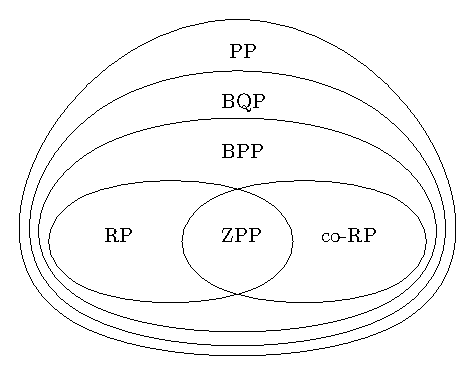
\includegraphics{img/rp-hierarchy.eps}
	\caption{Hierarchie pravděpodobnostních tříd}
\end{figure}

\vt P $\subseteq$ RP, ZPP $\subseteq$ RP

\tv (P ?= BPP) Je otevřený problém, zda P $=$ BPP. Pokud ano, pak P, RP, co-RP a
ZPP jsou si rovny.

\tv (Zero Polynomial Testing) Algoritmus na testování, zda je polynom ve více
proměnných roven nulovému polynomu, je v co-RP, ale  neví se, zda je v P.

\df (Monte Carlo, Las Vegas) Algoritmus, který běží v polynomiálním čase, ale
může vydat špatný výsledek, je {\bf Monte Carlo}. Algoritmus, který běží v
randomizovaném čase, ale vydá správný výsledek vždy, je {\bf Las Vegas}


\renewcommand{\arraystretch}{1.25}
\section{Grafové algoritmy}
\subsection{Nejkratší cesta}

Nejkratší cesty z jednoho vrcholu do všech ostatních (orientované grafy s
nezápornými váhami hran):

\begin{center}
\begin{tabular}{ l l p{8cm} }
	\hline
	\bf Algoritmus & \bf Čas & \bf Poznámka \\
	\hline
	Bellman-Ford & $\O(nm)$ & Funguje i v grafu se zápornými váhami. \\
	Dijkstra & $\O(n^2)$ & Funguje i v neorientovaných grafech. \\
	Dijkstra + FH & $\O(m + n\log n)$ & FH = Fibonacciho halda \\
	\hline
\end{tabular}
\end{center}

\noindent Nejkratší cesty mezi všemi dvojicemi vrcholů (orientované grafy bez záporných cyklů):

\begin{center}
\begin{tabular}{ l l p{8cm} }
	\hline
	\bf Algoritmus & \bf Čas & \bf Poznámka \\
	\hline
	Floyd-Warshall & $\O(n^3)$ & Funguje i v neorientovaných grafech. \\
	\hline
\end{tabular}
\end{center}

\subsection{Maximální tok}

Tj. algoritmy na hledání maximálního toku v síti ze zadaného vrcholu $s$
(zdroj), do zadaného vrcholu $t$ (stok). Velikost maximálního toku je navíc
rovna velikosti minimálního řezu.

\begin{center}
\begin{tabular}{ l l }
	\hline
	\bf Algoritmus & \bf Čas \\
	\hline
	Ford-Fulkerson & $\O(E\cdot \max_f)$\footnote{$\max_f$ je velikost maximálního toku} \\
    Edmonds-Karp & $\O(VE^2)$ \\
    Dinic & $\O(V^2E)$ \\
	Tři indové & $\O(V^3)$ \\
	Orlin + King, Rao, Tarjan & $\O(VE)$ \\
    \hline
\end{tabular}
\end{center}

\begin{itemize*}
\item \textbf{Ford-Fulkerson} hledá libovolnou zlepšující cestu.
\item \textbf{Edmonds-Karp} je Ford-Fulkerson, který hledá nejkratší
zlepšující cestu (pomocí BFS).
\item \textbf{Dinic} si staví vrstevnatou síť rezerv a v každém kroku jednu
hranu nasytí.
\item \textbf{Tři indové} počítají potenciál u vrcholů a v každém kroku
jeden vrchol nasytí.
\item \textbf{Orlin + King, Rao, Tarjan} je hodně složitý, dělal se celý
semestr na Semináři z grafových algoritmů.
\end{itemize*}

\subsection{Maximální párování}

\begin{center}
\begin{tabular}{ l l p{10cm} }
	\hline
	\bf Algoritmus & \bf Čas & \bf Poznámka \\
	\hline
	Edmonds & $\O(n^4)$ & Tzv. květinkový algoritmus. Později byla časová složitost zlepšena až na $\O(m\sqrt n)$ (Micali, Vazirani). \\
	Mucha, Sankowski & $\O(n^{2.376})$ & Randomizovaný, složitost je odvozena z násobení matic. \\
	\hline
\end{tabular}
\end{center}


\renewcommand{\arraystretch}{1.0}

\section{Algebraické a aritmetické algoritmy}
\subsection{Jednoduché algoritmy}
\begin{itemize}
	\item Strassenův algoritmus na násobení matic
	\item Euklidův algoritmus
	\item Eratosthenovo síto
\end{itemize}
\subsection{Prvočísla}

\vt (Lagrangeova) Pokud má konečná grupa $G$ podgrupu $H$, pak je řád $G$
dělitelný řádem $H$.
\vt (Malá Fermatova) Je-li $p$ prvočíslo a $\gcd(x,y) = 1$, potom platí $x^{p-1}
\equiv_y 1$.

\df (Eulerova funkce) Pro číslo $n$ definujeme $\varphi(n)$ počet čísel mezi $1$
a $n-1$ nesoudělných s $n$ (tj. $\gcd(n,i) = 1$.

\poz Některé vlastnosti Eulerovy funkce jsou:
\begin{itemize}
	\item $\varphi(n) = |\Z_n^*|$ (není samozřejmé)
	\item $\varphi(p) = p-1$ (z definice)
	\item $\varphi(ab) = \varphi(a) \cdot \varphi(b)$ pokud jsou $a$ a $b$
		nesoudělná
\end{itemize}
Speciálně, známe-li rozklad na prvočísla, je triviální podle posledních dvou
bodů vypočítat hodnotu funkce $\varphi$.

\vt (Eulerova) Pro libovolné $n > 0$ a $x$ s ním nesoudělné platí
$x^{\varphi(n)} \equiv_n 1$.

\poz Malá fermatova věta je speciální případ Eulerovy věty, kdy $n := p$.

\vt (O diskrétní odmocnině) Pokud je $p$ liché prvočíslo a $x \in \Z_p^*$, potom
má $x$ buďto právě dvě odmocniny, nebo nemá žádnou.

\vt (Čínská věta o zbytcích) Nechť $a_1, \dots, a_t$ jsou navzájem nesoudělná
čísla a $n = \prod a_i$, potom pro každé číslo $0 < x < n$ existuje právě jedna
$b$-tice zbytků $b_i = n \mod b_i$, tedy číslo je jednoznačně určené zbytky po
dělení $a_i$.

\alg (Fermatův test) Pro $n$ zvolíme $x$ uniformě náhodně mezi $2$ a $n-1$.
Spočteme $x^{n-1} \mod n$ a pokud vyjde $1$, prohlásíme $n$ za prvočíslo, jinak
za číslo složené.

\dk Pokud algoritmus odpoví, že je číslo složené, číslo $x$ je fermatův svědek,
který pomocí Malé fermatovy věty dokazuje složenost čísla. Abychom mohli Malou
Fermatovu větu použít, musí být $x$ a $n$ nesoudělné; pokud však soudělné jsou,
náš algoritmus stále odpoví správně a navíc výsledek výpočtu $x^{n-1}$ je
dělitelný společným dělitelem. \qed

\poz Bohužel existují čísla, říká se jim Carmichaelova, která Fermatova svědka
nemají a Fermatův test je nikdy neodhalí.

\vt Pokud $n$ není prvočíslo ani Carmichaelovo číslo, platí $x^{n-1} \equiv_n
1$ pro nanejvýš $n/2$ různých $x$.

\dk Označme všechna taková čísla jako $H$. Všechna jsou (z definice)
invertibilní, navíc jejich součin je taktéž v $H$; $H$ je tedy podgrupa $Z_n^*$,
a protože není číslo Carmichaelovo, musí $|H| \cdot k = \varphi(n) = |Z_n^*|$
pro nějaké $k \geq 2$ z Lagrangeho věty. \qed

\alg (Rabin-Miller) Nechť na vstupu je $n$, potom následující algoritmus na
prvočísla odpovídá správně a na složená čísla odpoví špatně s pravděpodobností
nanejvýš $1/4$.
\begin{enumerate}
	\item Vygeneruj náhodné $x: 1 < x < n$.
	\item Pokud $\gcd(x,n) \neq 1$, odpověz, že je číslo {\bf složené}.
	\item Najdi $t$ a liché $m$, t. ž. $n-1 = 2^t \cdot m$.
	\item Spočti $b_0 := x^m$ a $b_{i+1} := b_i^2$ pro $i\in \{1, \dots, t\}$.
	\item Pokud $b_t \equiv 1$, odpovíme, že je číslo {\bf složené} ($x$ je
		Fermatův svědek).
	\item Pokud jsou všechna $b_i \equiv 1$, odpovíme, že je číslo {\bf
		prvočíslo}.
	\item Jinak pro nejvyšší $i$ takové, že $b_i \not\equiv 1$, pokud je $b_i
		\equiv -1$ odpovíme, že je číslo {\bf prvočíslo}, jinak {\bf složené}.
\end{enumerate}

\pzn (Derandomizace) Pokud by se ukázalo, že platí Riemannova hypotéza (Grupa je
generována svými $\O(\log^2 n)$ nejmenšími prvky), stačilo by testovat tyto
generátory (protože všechna $x$, která o prvočíslu lžou, jsou v generátoru -- to
ale není triviální ukázat). Tedy pokud ještě určíme, jaká je konstanta v $\O$,
což by ale mělo být $2$.

\alg (RSA) Nechť $p,q$ jsou dvě velká prvočísla, $n := p \cdot q$, $y = x^{-1}$
náhodný reverzibilní prvek a jeho inverzi modulo $\varphi(n)$. Potom lze
šifrovat pomocí $a^x \mod n$ a dešifrovat pomocí $a^y \mod n$.

\dk (Pouze pro $\gcd(a,n) = 1$) Počítejme: $a^{xy} = a^{1 + k\varphi(n)}$,
protože $xy \equiv_{\varphi(n)} 1$. Ale to je rovno po vytknutí $1$ z exponentu
$a \cdot a^{k\varphi(n)} = a \cdot (a^{\varphi(n)})^k = a$ podle Eulerovy věty.

\section{Teorie mnohostěnů}
\subsection{Roviny, nadroviny, mnohostěny}

\df (Nadrovina) V $\R^n$ je nadrovina množinou všech $x$ takových vektorů, kde
se zafixuje jedna (nebo více) složek vektoru. Matematicky tedy: $\{x \in \R^n:
a^Tx = b\}$ pro nějaké $a \in \R^n$, kde $a \neq 0$ a $b \in R$ (nulový vektor by generoval
celý prostor, třeba napíšeme jedničku do skožky $a$, kterou chceme zafixovat,
a její požadovanou hodnotu do $b$).

\poz Všimneme si, že pokud chceme fixovat více souřadnic, tak to neznamená, že
se jejich hodnoty zafixují, ale spíše jejich součet (podle hodnoty $a$). To ale
ve skutečnosti chceme, tím se totiž dá vyrobit nadrovina, která má jiný
\uv{sklon}, než kolmý na jednu osu.

\df (Poloprostor) V $\R^n$ je poloprostor množina všech $x$ takových vektorů,
které jsou \uv{na jedné straně nadroviny}, matematicky tedy:  $\{x \in \R^n:
a^Tx \leq b\}$ pro nějaké $a \in \R^n, a \neq 0, b \in \R$.

\df (Konvexní mnohostěn) Konvexní mnohostěn v $\R^n$ je množina, kterou lez
vyjádřit jako průnik konečně mnoha poloprostorů.

\poz Může se snadno stát, že mnohostěn sice bude konvexní, ale nebude omezený.

\vt (Oddělovací) Nechť množiny $C,D \subseteq \R^n$ jsou uzavřené, konvexní a disjunktní
a $C$ navíc omezená. Pak existuje nadrovina, která silně odděluje $C$ a $D$, tj.
$C \subseteq \{x | a^Tx < b\}$ a $D \subseteq \{x | a^T x > b\}$.

\dk Seženeme si $c \in C$ a $d \in D$ takové, že jejich vzdálenost je minimální.
Jediný problém může být, když nebude $D$ omezená. V takovém případě můžeme ale
vybrat nějaký bod $d'\in D$, nejvzdálenější bod k němu v $c'\in C$ a potom
udělat kružnici se středeme v $c'$ protínající $d'$; průnik této kružnice s $D$
nám výběr potřebně omezní a z výběru $c'$ a $d'$ je zřejmé, že správný bod v ní
bude ležet (jinak jsem špatně vybral nejvzdálenější $c'$).

Pak stačí vzít vektor $(c,d)$ jako normálu naší nadroviny, a ukotvit ji třeba na
půli cesty mezi $c$ a $d$:
\begin{align}
	a &:= d - c \\
	b &:= a^T\left({c+d \over 2}\right)
\end{align}

\df (Kužel) Nechť $a_i\in R^n$ jsou vektory. Potom definujeme kužel $C$ jako
konvexní obal polopřímek vycházejících z počátku a procházejících body $a_i$.

\lm (Farkas) Nechť $a_1, \dots, a_n, b \in \R^m$. Pak nástane jedna z možností:
\begin{enumerate}
	\item Bod $b$ leží v kuželu definovaným $a_i$.
	\item Existuje nadrovina $h$ procházející počátkem, tvaru $h = \{x \in \R^m
	: y^Tx = 0\}$, oddělující bod $b$ od kuželu definovaného $a_i$.
\end{enumerate}
\dk Pokud je $b$ v kuželu, je hotoov. Jinak nadrovinu můžeme najít pomocí
oddělovací věty aplikované na $b$ a kužel. Ta nám sice nedá nadrovinu nutně
procházející počátkem, ale protože je kužel konvexní a nadrovina $b$ odděluje
od kuželu, můžeme ji do počátku posunout a kužel stále protínat nebude. \qed

Dále se nám bude hodit ale více algebraické vyjádření:

\lm (Farkas) Soustava nerovnic $Ax \leq b$ má nezáporné řešení $x$ právě, když
každé nezáporné $y$, pro než $y^TA \geq 0^T$ splňuje také $y^Tb \geq 0$.

\subsection{Lineární programování}

\df (Standardní tvar) Úloha LP je ve standardním tvaru, pokud je tvaru:
\begin{align}
	\max_x c^Tx : \quad Ax \leq b
\end{align}

\df (Rovnicový tvar) Úloha LP je v rovnicovém tvaru, pokud je tvaru:
\begin{align}
	\max_x c^Tx : \quad Ax = b, \quad x \geq 0
\end{align}

Tedy jediná nerovnice, je podmínka na nezápornost vektoru $x$. Máme-li obecnou
úlohu LP, můžeme ji celkem snadno do tohoto tvaru převést, nerovnice totiž lze
nahradit přidáním dalších proměnných a konstant tak, aby stačila nezápornost.

Pro simplexovou metodu chceme rovnicový tvar, pro geometrickou představu nám
bude ale milejší stadardní tvar, protože svou podobou každá nerovnice přímo
vyjadřuje nějakou nadrovinu, a tedy jejich průnik nám tvoří mnohostěn!

\df (Bázické řešení) Vektor $x \in \R^n$ je bázické přípustné řešení úlohy LP v
rovnicovém tvaru, pokud je $x$ přípustné řešení a existuje $B \subseteq \{1,
\dots, n\}$ taková, že čtvercová matice $A_B$ (sloupečky indexované $B$) je
regulární a $x_j = 0$ kdykoliv $j \notin B$.

\tv (Unikátnost bázických řešení) Pro každou množinu $B$ existuje nanejvýš jedno
přípustné bázické řešení $x \in \R^n$.

\dk Kdykoliv máme $B$, matice $A_B$ je regulární a tedy soustava $A_B x_B = b_B$
právě jedno řešení. Podmínka pro přípustné bázické řešení navíc říká, že ostatní
prvky $x_{\overline{B}}$ musí být nulové. \qed

\df (Báze) Množině $B$ budeme říkat báze. Pokud navíc určuje přípustné řešení,
budeme jí říkat {\it přípustná báze}.

\vt (O existenci optimálního řešení) Pro program v rovnicovém tvaru platí:
\begin{enumerate}
	\item Pokud existuje alespoň jedno přípustné řešení a účelová funkce je na
	množině všech přípustných řešení shora omezená (pro minimalizační zdola),
	pak existuje také optimální řešení.
	\item Existuje-li optimální řešení, potom i některé z bázickcýh přípustných
	řešení je optimální.
\end{enumerate}
\dk Trošku technický, stačí ale dokázat, že pokud je účelová funkce omezená, pro
libovolné řešení $x_0$ existuje lepší bázické řešení $x_b$, které je alespoň tak
dobré.

To nám samo o sobě dává informaci, jak řešit lineární programy: stačí projít
všechny báze, vyřešit pro každou z nich soustavu rovnic, a hledat
nejlepší řešení. Bohužel, bazí je exponenciálně mnoho, abychom to dělali hloupě.

{\it Simplexová metoda} je chytrý způsob, jak řešit lineární programy. Typicky
začíná s nějaký bázickým řešením a s vědomostí, že existuje optimální bázické řešení,
se k němu snaží dospět postupným vylepšováním účelové funkce. Ačkoli je to
metoda v praxi rychlá, nikde není záruka, že běží v polynomiálním čase --
bohužel se může stát, že před nalezením optima projde většinu bazických řešení.


\vt (O Dualitě LP) Pro dvě úlohy LP:
\begin{align}
\tag P
\label{dualita:P}
	\max c^Tx&: \quad Ax \leq b, \quad x \geq 0 \\
\tag D
\label{dualita:D}
	\min b^Ty&: \quad A^T y \geq c, \quad y \geq 0
\end{align}
nastane jedna z následujících možností:
\begin{enumerate}
	\item Ani jedna z úloh nemá přípustné řešení.
	\item Jedna z úloha je neomezená, druhá nemá přípustné řešení.
	\item Obě úlohy mají přípustné řešení, a navíc pro optimální řešení $x^*$ a
	$y^*$ platí $c^T x^* = b^Ty^*$.
\end{enumerate}

\dk Použijeme Farkasovo Lemma. Nechť $\gamma = c^Tx^*$ je hodnota účelové funkce
pro nějaké optimální řešení \eqref{dualita:P}. Pro $\epsilon \geq 0$ má tedy z
definice optima systém $Ax \leq b, c^Tx \geq \gamma + \epsilon$ přípustné řešení právě pro
$\epsilon = 0$. Farkasovo lemma ale neví nic o účelové funkci. Nevadí, přidáme
ji jako řádek do naší matice $A$ a optimalitu vyjádříme jako $\gamma + \epsilon$
v jedné složce pravé strany!
\begin{align}
	A' = \left(\begin{array}{c} A \\ -c^T \end{array}\right), \quad b' =
	\left(\begin{array}{c} b \\ -\gamma - \epsilon\end{array}\right)
\end{align}
A to již můžeme poslat do lemmatu a protože víme, že pro $\epsilon > 0$ žádné
nezáporné řešení neexistuje. Musí tedy existovat nějaký nezáporný vektor $y'$, že
$y'^TA' \geq 0$, ale $y'^T b' < 0$. To ale můžeme dát dohromady a levou stranu
transponovat:
\begin{align}
	y^TA' \geq 0 > y^T b' \qquad \Rightarrow \qquad
	A'^Ty \geq b'^T y
\end{align}
Co to znamená? Pamatujme, že cílovou funkci máme zakódovanou ve vektoru
$y'$, dává nám to tedy nějaké řešení duálního programu, které je jenom o epsilon
menší, než optimum primáru. Protože to můžeme udělat pro libovolně malé
$\epsilon$, musí si být rovny.
\qed


\section{Problém obchodního cestujícího}

Problém obchodního cestujícího budeme zkracovat na TSP, z anglického názvu
Travelling salesman problem. Úkolem je najít nejkratší cestu, která navštíví
všechny města a vrátí se zpět do prvního, za předpokladu, že mezi každými dvěma
městy vede silnice. V řeči teorie grafů můžeme problém definovat následovně.

\medskip
\noindent\textbf{Optimalizační verze:} V daném ohodnoceném úplném grafu najděte
nejkratší Hamiltonovskou kružnici. 

\noindent\textbf{Rozhodovací verze:} Existuje v daném ohodnoceném úplném grafu
Hamiltonovská kružnice kratší než $k$?
\medskip

Obecně nemusí platit trojúhelníková nerovnost, ale předpokládáme, že váhy
jednotlivých hran jsou nezáporné.

\subsection{Obtížnost TSP}

\vt TSP je $\NP$-úplný.

\dk Převodem na Hamiltonovskou kružnici v grafu $G = (V,E)$. Hranám úplného
grafu, které jsou v $E$ přiřadíme váhu 1, hranám které nejsou v $E$ váhu 2 a
ptáme se, zda existuje řešení TSP s váhou $|V|$. TSP $\in \NP$ dokážeme tak, že
použijeme výsledné pořadí vrcholů jako certifikát.\footnote{Řešíme rozhodovací
verzi, takže stačí ověřit, že je to kružnice s délkou nejvýše $k$ -- nemusíme
ověřovat, že je nejkratší, to by samozřejmě bylo těžší.}

Z toho, že TSP je $\NP$-úplný je jasné, že neznáme žádný polynomiální
deterministický algoritmus, který by TSP řešil. Známe ale několik aproximačních
algoritmů, které najdou přijatelně dobré (i když ne nejlepší) řešení.

\subsection{Aproximační algoritmy na TSP}

Všechny aproximační algoritmy pro TSP předpokládají, že platí trojúhelníková
nerovnost.

\alg (Aproximace přes kostry) Nejprve najdeme minimální kostru grafu $G$. Ta je
dolním odhadem na řešení TSP.\footnote{Kdyby bylo řešení TSP menší, než
minimální kostra, pak bychom dostali menší kostru vypuštěním libovolné hrany z
řešení TSP.} Začneme z libovolného vrcholu a určíme pořadí vrcholů tak, že
půjdeme okolo rovinného nakreslení minimální kostry po směru hodinových ručiček.
Toto pořadí vrcholů vydáme jako výsledek.

\vt Aproximace přes kostry je polynomiální 2-aproximační algoritmus pro TSP s
trojúhelníkovou nerovností.

\alg (Christofides)
\begin{enumerate*}
\item Nalezneme minimální kostru $T$ grafu $G$.
\item Označme $O$ vrcholy s lichým stupněm v $T$. Nalezneme perfektní párování
$M$ na vrcholech $O$ s minimální váhou.
\item Sjednotíme $T$ a $M$ a získáme multigraf $H$.
\item Najdeme Eulerovský tah v $H$ ($H$ je souvislý a má stupně všech vrcholů sudé).
\item Vytvoříme Hamiltonovskou kružnici tak, že půjdeme po Eulerovském tahu a
budeme přeskakovat již navštívené vrcholy.
\end{enumerate*}

\vt Christofides je polynomiální $3\over 2$-aproximační algoritmus pro TSP s
trojúhelníkovou nerovností.

\dk Všimněme si nejprve, že přeskakováním již navštívených vrcholů nikdy
nedostaneme delší cestu, což plyne z trojúhelníkové nerovnosti.

Označme $A$ množinu hran, která je optimálním řešením TSP v úplném grafu $G =
(V,w)$. Protože graf $(V,A)$ je souvislý, obsahuje nějakou kostru $T$ a zjevně
$w(A) \ge w(T)$. Označme $B$ množinu hran, která je optimálním řešením TSP v
úplném grafu $(O,w)$. Protože platí trojúhelníková nerovnost, musí být $w(A) \ge
w(B)$.

Ukážeme, že existuje perfektní párování na $O$, které váží méně než $w(B)/2 \le
w(A)/2$. $O$ jistě obsahuje sudý počet vrcholů, tedy existuje maximální
párování. Vezmeme graf $(O,B)$, který sestává právě z jedné Hamiltonovské
kružnice. V této kružnici vezmeme buď všechny liché hrany, nebo všechny sudé
hrany a prohlásíme je za párování. Protože váha celé kružnice je $w(B)$, pak
váha lichých nebo sudých hran musí být nejvýš $w(B)/2$. Tedy, $w(M) + w(T) \le
w(A) + w(A)/2$ a algoritmus je $3\over 2$-aproximační. 
\qed





\section{Speciální matice}

\subsection{Pozitivně definitní matice}

\df \emph{Pozitivně definitní matice} je čtvercová matice $M$, pro kterou platí
$$\mathbf{x} \neq 0 \Rightarrow \mathbf{x}^TM\mathbf{x} > 0$$
Pozitivně definitní matice má vždy kladná vlastní čísla. Naopak, každá
symetrická matice, jejíž vlastní čísla jsou kladná, je pozitivně definitní.
Obecněji můžeme definovat pozitivně definitní matici v oboru komplexních čísel.

\df \emph{Pozitivně definitní matice} je hermitovská\footnote{V hermitovské
matici platí, že $M_{ij} = \overline{M_{ji}}$, tedy že na symetrickém místě se
nachází číslo komplexně sdružené. Stejně tak zobecněná transpozice $\mathbf{z}^*
= \mathbf{\bar z}^T$.} matice $M$, pro kterou platí
$$\mathbf{z} \neq 0 \Rightarrow \mathbf{z}^*M\mathbf{z} > 0$$

Analogicky můžeme definovat i negativně definitní matice.

\subsection{Pozitivně semidefinitní matice}
\df \emph{Pozitivně semidefinitní matice} je čtvercová matice $M$, pro kterou platí
$$\forall \mathbf{x} \in \C^n:\quad \mathbf{x}^*M\mathbf{x} \ge 0$$

Analogicky můžeme definovat i negativně semidefinitní matice.

\todo Láďa: formulace semidefinitního programování + příklad MAXCUT, souvislost
s elipsoidovou metodou.

\subsection{Hadamardovy matice}

\df Hadamardova matice je čtvercová matice s hodnotami pouze $+1$ a $-1$, jejíž
řádky jsou po dvou ortogonální.

Mezi zajímavé vlastnosti Hadamardovy matice patří:

\begin{itemize*}
\item $HH^T = n\In$ (plyne triviálně z ortonormality).
\item $\det(H) = \pm n^{n\over 2}$ Navíc má Hadamardova matice v absolutní
hodnotě největší determinant ze všech matic, jejichž prvky nabývají hodnot z
intervalu $[-1, 1]$.
\item Každé dva řádky mají přesně polovinu hodnot v odpovídajících sloupcích stejných a polovinu opačných.
\end{itemize*}

\tv Řád Hadamardovy matice musí být 1, 2, nebo násobek 4.

\alg (Silvestrova konstrukce) Mějme Hadamardovu matici $H$ řádu $n$. Potom
$$\begin{pmatrix}
H & H \\
H & -H
\end{pmatrix}$$
je Hadamardova matice řádu $2n$.

Zobecněním této konstrukce můžeme dojít k odvození, že mám-li Hadamardovy matice
řádu $n$ a $m$, dokážeme zkonstruovat Hadamardovu matici řádu $nm$. Ani to nám
ale ještě nestačí na všechny násobky 4.

\conj \emph{(Hadamard conjencture)} Pro každé $k \in \Z^+$ existuje Hadamardova
matice řádu $4k$.

\smallskip
Nejmenší Hadamardova matice, o níž se zatím neví zda existuje, je řádu 668.

\smallskip
Hadamardovy matice se používají v samoopravných kódech, v tzv. Hadamardově kódu.
Ten se používá všude tam, kde hrozí velký šum a nespolehlivost přenosového
kanálu. Byl např. použit v roce 1971 pro přenos fotografií Marsu zpět na zem ze
sondy Mariner 9.

\smallskip\noindent\textbf{Hadamardův kód} mapuje zprávy délky $k$ v binární
abecedě na kódová slova délky $2^k$, přičemž minimální vzdálenost kódu je
$2^k/2$. Kódová slova získáme jako řádky $H_n$ a $-H_n$ a nahrazením všech
$1$ za $0$ a $-1$ za $1$. Tak získáme $2n$ kódových slov délky $n = 2^k$.

Existuje i varianta Hadamardova kódu s kódovými slovy délky $2^{k-1}$ a
minimální vzdálenosti $2^{k-2}$, který je v praxi používán častěji, neboť při
stejné relativní vzdálenosti používá kratší kódová slova.

\tv Pro délku bloku zprávy $k \le 7$ jsou Hadamardovy kódy optimální vzhledem k
minimální vzdálenosti kódu.

\subsection{Totálně unimodulární matice}

\df (Totálně unimodulární matice) Matice je totálně unimodulární, pokud jsou
determinanty všech jejích čtvercových podmatic rovny $0$, $1$ nebo $-1$.

Více o aplikacích v sekci \ref{LP:celociselnost}, v rámci celočíselnosti LP.

\section{Celočíselnost}
\label{LP:celociselnost}
\df (Celočíselný LP) Lineární program nazveme celočíselným, pokud k němu přidáme
podmínku, aby všechny proměnné byly celočíselné. Pro celočíselné programy budeme
používat zkratku ILP (Integer Linear Program).

Je zřejmé, že ILP nemusí jít řešit polynomiálně, například protože je snadné
najít redukci ze SATu na ILP. Nadruhou stranu ale není důvod, proč by jednodušší
programy nemohly jít řešit polynomiálně. 

\tv Pro LP \eqref{LP:max-bipartitni-parovani} řešící perfektní párování v bipartitním grafu platí, že pro každé
optimální řešení existuje alespoň jedno stejně dobré řešení celočíselné.

\begin{align}
\label{LP:max-bipartitni-parovani}
&\max \sum_{e \in E} w_e x_e: \quad \sum_{e \in E: v \in e} x_e = 1 \forall v
	\in V, \quad x_e \in \{0, 1\} \\
	\text{relaxace:}\qquad	&\max \sum_{e \in E} w_e x_e: \quad \sum_{e \in E: v \in e} x_e = 1 \forall v
	\in V, \quad 0 \leq x_e \leq 1
\end{align}

\dk Nechť máme nějaké řešení, které má neceločíselné
složky. Začněme tedy s nějakou neceločíselnou hranou a najdeme cyklus (sudý,
jiné v bipartitním grafu nejsou) neceločíselných hran. Takový existuje, protože
suma každého vrcholu je 1 a vstoupili jsme z neceločíselného. Na cyklu poté pro
nějaké $\epsilon$ změníme váhy, pro lichou hranu $+$, pro sudou $-$. To
zachovává optimalitu, zvolíme tedy $\epsilon$ největší, aby zachovávalo také
přípustnost. Protože ale suma na každém vrcholu zůstává stejná, znamená to, že
některá hrana narazila na hranici $0$ nebo $1$. Máme tedy optimální řešení,
které má méně neceločíselných hodnota. Takto můžeme pokračovat, dokud žádné
takové nejsou. \qed

Existuje ale nějaké obecné tvrzení, které by nám zaručovalo podobnou hezkou
vlastnost? Odpovědí jsou totálně unimodulární matice.

\df (Totálně unimodulární matice) Matice je totálně unimodulární, pokud jsou
determinanty všech jejích čtvercových podmatic rovny $0$, $1$ nebo $-1$.

\poz Pokud je $A$ totálně unimodulární, potom také $A^T$ je totálně
unimodulární.

\vt (O celočíselnosti LP) Nechť $\max c^Tx : Ax = b$ je lineární program, $A$ je totálně
unimodulární matice a $b$ je celočíselné. Potom všechna bazická řešení tohoto
programu jsou celočíselná.

\dk Pro nějaké řešení existuje báze $B$. Vezmeme si matici $A_B$ a víme, že pro
nějaký vektor $x'$ platí $A_Bx_B = b_B$. Pokud je determinant $A_B$ nenulový
(což je, jinak by to nebyla báze), můžeme použít Cramerovo pravidlo na výpočet
$x_i = \det((A_B)_i) / \det_(A_B)$. Tady $(A_B)_i$ je matice, kde $i$-tý
sloupeček byl nahrazen vektorem $b_i$. Nyní stačí říct, že jmenovatel je $\pm1$
z totální unimodularity a čitatel můžeme spočítat třeba rozvojem podle sloupečku
$i$, a opět z totální unimodularity máme v každém kroku celočíselné hodnoty.
\qed

Takže totálně unimodulární matice nám dávají záruku, že všechny bazické
řešení (tedy takové, které vydá simplexová metoda) jsou celočíselné. Jak ale
poznáme, že je matice totálně unimodulární?

\vt Matice $A$ je totálně unimodulární právě tehdy, když pro každou podmnožinu
řádků matice $X$ lze rozdělit tyto řádky na skupiny $\cdot 1$ a $\cdot -1$ tak,
aby součet každého sloupečku byl $0$ nebo $\pm 1$.

\poz Matice incidence bipartitního grafu je totálně unimodulární: Nechť řádky
jsou vrcholy a sloupečky hrany. Pak každý sloupeček má součet právě $2$. V
libovolném obarvení nám tedy stačí, když řádky budou obarveny dle partity a
součet bude $0$; pokud některý řádek hraně bude chybět, součet bude $\pm1$.

\poz Matice incidence orientovaného grafu je totálně unimodulární: Všechny řádky
můžeme obarvit stejně, protože součet sloupečku je vždy $0$ a skládá se právě z
jedné $1$ a jedné $-1$.

\section{Párování a toky v sítích}
\section{Teorie matroidů}

Matroid je struktura v kombinatorice, která zobecňuje koncept
\uv{nezávislosti}, jehož konkrétním příkladem je lineární nezávistlost ve
vektorových prostorech. Existuje mnoho ekvivalentních způsobů jak zavést
matroidy, nejvýznamnějšími jsou nezávislé množiny, báze, kružnice a ranková
funkce. Teorie matroidů si často vypůjčuje teminologii z lineární algebry a
teorie grafů.

\subsection{Definice přes nezávislé množiny}
\df Matroid $M$ je dvojice $(S,I)$, kde $S$ je konečná množina (nazýváme ji
\emph{nosná množina} a $I \subset 2^S$ je množina podmnožin $S$ (nazýváme je
nezávislé množiny), splňující následující vlastnosti:
\begin{enumerate*}
\item Prázdná množina je nezávislá, tedy $\emptyset \in I$.
\item Každá podmnožina nezávislé množiny je nezávislá, tedy pro každé $A' \subseteq A \subseteq S$ platí $A \in I \Rightarrow A' \in I$. Tato vlastnost se nazývá \emph{dědičnost}.
\item Pokud $A$ a $B$ jsou dvě nezávislé množiny z $I$, $|A| = |B| + 1$, pak existuje prvek $x\in A\setminus B$ tž. $B\cup\{x\}$ je nezávislá. Tato vlastnost se nazývá \emph{výměnná vlastnost}.
\end{enumerate*}

\df Podmnožina $S$, která není v $I$ se nazývá \emph{závislá}. Maximální nezávislá
množina (po přidání libovolného prvku se stane závislou) se nazývá \emph{báze}.
Naopak minimální závislou množinu (po odebrání libovolného prvku se stane
nezávislou) nazýváme \emph{kružnice}.

\pzn Grafová analogie: $S$ je množina hran grafu, $I$ je množina všech lesů na
hranách $S$. Báze odpovídá kostře grafu $G$, kružnice cyklu v grafu $G$.

\pzn Vektorová analogie: $S$ je množina sloupců matice. Nezávislé množiny jsou
pak právě lineárně nezávislé množiny vektorů z $S$. Báze matroidu odpovídají
bázím vektorového prostoru. 

\subsection{Definice přes báze}
\df Matroid $M$ je dvojice $(S,\B)$, kde $S$ je konečná množina a $\B$ je
množina podmnožin $S$ (tyto podmnožiny nazýváme báze), splňující následující
vlastnosti:
\begin{enumerate*}
\item $\B$ je neprázdná.
\item Když $A,B \in \B$ jsou různé a $a \in A\setminus B$, pak existuje $b \in B\setminus A$ tž. $A\setminus\{a\}\cup\{b\} \in \B$.
\end{enumerate*}

\poz Tato definice je ekvivalentní s definicí přes nezávislé množiny. Nezávislé
množiny jsou právě podmnožiny bází.

\subsection{Definice přes kružnice}
\df Matroid $M$ je dvojice $(S,\c)$, kde $S$ je konečná množina a $\c$ je
množina podmnožin $S$ (tyto podmnožiny nazýváme kružnice), splňující
následující vlastnosti: 
\begin{enumerate*}
\item $\emptyset \notin \c$
\item Pokud $A$ i $B$ jsou kružnice, pak $A\subseteq B \Rightarrow A = B$.
\item Když $A$ i $B$ jsou kružnice a $e\in A\cap B$, pak existuje kružnice v $A\cup B$, která neobsahuje $e$.
\end{enumerate*}

\poz Tato definice je ekvivalentní s definicí přes nezávislé množiny. Nezávislé
množiny jsou právě ty, které neobsahují žádnou kružnici.

\subsection{Definice přes rankovou funkci}
\df Ranková funkce je zobrazení $r: 2^S \rightarrow \N$, která každé podmnožině
$S$ přiřadí velikost její největší nezávislé podmnožiny.

\df Matroid $M$ je dvojice $(S,r)$, kde $S$ je konečná množina a $r: 2^S
\rightarrow \N$ je ranková funkce, splňující následující vlastnosti:
\begin{enumerate*}
\item $0 \le r(X) \le |X|$
\item $X\subseteq Y \Rightarrow r(X) \le r(Y)$
\item $r(X\cup Y) + r(X\cap Y) \le r(X) + r(Y)$
\end{enumerate*}

\poz Tato definice je ekvivalentní s definicí přes nezávislé množiny. Nezávislé množiny jsou právě ty, kde $r(X) = |X|$.

\subsection{Přehled jednoduchých vlastností}
\tv Všechny báze matroidu $M$ mají stejnou velikost $r(M)$. Toto číslo
označujeme jako rank matroidu $M$. V grafech je zjevně $r(G) = n-k$, kde $n$ je
počet vrcholů a $k$ počet komponent.

\df Duální matroid $M^*$ definujeme tak, že jeho báze jsou doplňky bází $M$.
Pak zjevně platí $M^{**} = M$.

\df Smyčka je prvek $S$, který není obsažen v žádné bázi. Co-smyčka je prvek
$S$ obsažený v každé bázi.

\df Uniformní matroid $U_{k,n}$ na $n$ prvcích definujeme tak, že nezávislými
podmnožinami jsou právě ty, jejihž velikost je nejvýše $k$. V $U_{0,n}$ je
každý prvek smyčka, v $U_{n,n}$ je každý prvek co-smyčka.

\subsection{Operace s matroidy}
\df Nechť $M = (S_1,I_1)$ a $N = (S_2,I_2)$ jsou matroidy. \emph{Direktní
součet} matroidů $M$ a $N$ je matroid $(S_1 \sqcup S_2, I_1 \sqcup I_2)$, kde
$A\sqcup B$ značí disjuktní sjednocení množin $A$ a $B$.

\df Nechť $M = (S_1,I_1)$ a $N = (S_2,I_2)$ jsou matroidy. \emph{Sjednocení
matroidů} $M$ a $N$ je matroid $(S_1\cup S_2, \{i_1\cup i_2 ~|~ \forall i_1\in
I_1, \forall i_2\in I_2\})$.

\subsection{Hladový algoritmus}
\df \emph{Systém nezávislých množin} je dvojice $(S,I)$, kde $S$ je konečná
množina a $I \subset 2^S$ je množina podmnožin $S$ (nazýváme je nezávislé
množiny), splňující, že $\emptyset\in I$ a každá podmnožina nezávislé množiny
je též nezávislá.

\vt Mějme $M = (X,J)$ systém nezávislých množin a orákulum, které nám pro každou
množinu $Y\subseteq X$ určí, zda je nezávislá. Definujeme hladový algoritmus
tak, že začne s prázdnou množinou $S$ a poté do ní v každém kroku přidá prvek z
$X$ s nejnižším ohodnocením, který neporuší nezávislost $S$. Potom hladový
algoritmus vygeneruje maximální nezávislou množinu $S$ s minimálním součtem
ohodnocení pro každou nezápornou ohodnocovací funkci $w: X \rightarrow \N$ právě
tehdy, když $M$ je matroid.

\dk Rozdělíme tvrzení na dvě implikace a dokážeme každou zvlášť.

\noindent \textbf{1) $M$ je matroid $\Rightarrow$ hladový algoritmus funguje pro
každé ohodnocení $w$}

Je zjevné, že hladový algoritmus nalezne maximální nezávislou množinu. Vezměmě
výstup hladového algoritmu $\{x_1,\dots,x_r\}$ tž. $w(x_1) \le \dots \le
w(x_r)$. Pro spor předpokládejme, že existuje nezávislá množina
$\{y_1,\dots,y_r\}$ tž. $w(y_1) \le \dots \le w(y_r)$ a $w(x_k) > w(y_k)$
pro nějaké $k$. Pokud by takové $k$ neexistovalo, je $\{x_1,\dots,x_r\}$
maximální nezávislá množina s minimálním ohodnocením.

Předpokládejme, že $k$ je nejmenší takové, že $w(x_k) > w(y_k)$. Zjevně $k > 1$.
Potom mějme $S = \{x_1,\dots,x_{k-1}\}$ a $T = \{y_1,\dots,y_k\}$. Platí, že
$|T| = |S|+1$ a tedy podle výměnné vlastnosti matroidů existuje $j \in
\{1,\dots,k\}$ tž. $S\cup \{y_j\}$ je nezávislá množina (a $y_j$ není v $S$).
Protože $w(y_j) \le w(y_k) < w(x_k)$, hladový algoritmus by vybral $y_j$ dříve,
než $x_k$, což je spor.

\noindent \textbf{2) hladový algoritmus funguje pro každé ohodnocení $w$
$\Rightarrow$ $M$ je matroid}

Předpokládejme, že máme systém nezávislých množin, který nesplňuje výměnnou
vlastnost. Zkonstruujeme ohodnocovací funkci $w$ takovou, že na ní hladový
algoritmus selže. Mějme tedy $A,B \subset X$ nezávislé množiny takové, že $|A| =
|B| + 1$, ale pro žádné $a \in A\setminus B$ není $B\cup \set a$ nezávislá
množina. Pak definujme:
\begin{align*}
w(x) = \left\{
	\begin{array}{lr}
		w_1\quad\text{pokud}~x \in A\cap B \\
		w_2\quad\text{pokud}~x \in B \setminus A \\
		w_3\quad\text{pokud}~x \in A \setminus B \\
		w_4\quad\text{jinak}
	\end{array}
	\right.
\end{align*}

Dále definujme, $w_1 < w_2 < w_3 < w_4$. Všimněme si, že hladový algoritmus
nejprve vybere všechny prvky z $A\cap B$, poté všechny prvky z $B\setminus A$ a
pak (podle předpokladu) už nebude moci vybrat žádný prvek z $A\setminus B$.
Protože $B$ není maximální, budeme k němu muset přidat prvek z
$X\setminus\set{A\cup B}$, který má váhu $w_4$.

Nyní nám stačí nastavit konstanty $w_1,\dots,w_4$ tak, aby byl výsledek
hladového algoritmu těžší, než kterákoliv nezávislá množina obsahující $A$
(taková zjevně musí existovat). Mějme tedy $m$ velikost maximální nezávislé
množiny. Chceme:
\begin{align*}
|A\cap B|w_1 + |B-A|w_2 + (m-|B|)w_4 > |A\cap B|w_1 + |A-B|w_3 + (m-|A|)w_4
\end{align*}
Protože $|A| = |B|+1$, tak:
\begin{align}
\label{rov:hungry-w4}
w_4 > |A-B|w_3 - |B-A|w_2
\end{align}
Hladový algoritmus vybere o jeden prvek s váhou $w_4$ více, než kdyby nejdříve
pobral celou množinu $A$. Musíme tedy nastavit $w_4$ dostatečně velké. Jeden ze
způsobů, jak jej zvolit (pro libovolné $\varepsilon\in (0,1)$):
\begin{align*}
w_1 &= \varepsilon /|X| \\
w_2 &= \varepsilon /|B-A| \\
w_3 &= (1+\varepsilon) /|A-B| \\
w_4 &= 2
\end{align*}

Pak už stačí jen dokázat, že takto zvolená $w$ splňuje $w_1 < w_2 < w_3 < w_4$ a
že platí rovnice \ref{rov:hungry-w4}.
\qed

\subsection{Matroid intersection theorem}
\todo



\section{Elipsoidová metoda}
{\it Trošku širší úvod lze nalézt ve skriptíčkách J. Matouška: Lineární
programování a lineární algebra pro informatiky, ITI série 2006-311.}

Elipsoidová metoda je výrazná proto, že jako první dala polynomiální odhad na
řešení lineárních programů. Její praktičnost ale mírně pokulhává, za chvíli bude
jasné proč.

\alg (Elipsoidová metoda) Pro LP $\max c^Tx: Ax \leq b$, $R$ a $\varepsilon$
definujeme algoritmus, který vrátí nějaký bod polyedru $P$ definovaného rovnicí $Ax \leq b$,
pokud tento polyedr obsahuje kouli velikosti alespoň $\varepsilon$.
\begin{enumerate}
	\item Začni s koulí $E_0 := B(0, R)$ (předpokládáme, že $P \subseteq E_0$).
	\item V kroku $k$ nechť $s_k$ je střed elipsoidu $E_k$. Pokud $s_k \in P$,
	vrať $s_k$ jako výsledek a skonči.
	\item Jinak zvol nějakou porušenou nerovnost, označ $H_k$ jako půlelipsoid
	$E_k$ vyhovující porušené nerovnosti a najdi elipsoid $E_{k+1}$, který má
	nejmenší objem takový, že obsahuje $H_k$.
	\item Je-li objem $E_{k+1}$ menší, než objem koule o poloměru $\varepsilon$,
	oznam že úloha nemá řešení a skonči. Jinak pokračuj krokem 2.
\end{enumerate}
Tento algoritmus provede zhruba $\O(n^2\log (R/\varepsilon))$ iterací.

Když pomineme spoustu chlupatých problémů, které je potřeba v algoritmu vyřešit
(například jak se poprat s elipsoidama, které nevypadají, že by měly racionální
parametry), zbývá ještě vyřešit pár problémů.

Například algoritmus jak je popsaný vůbec nebere v úvahu účelovou funkci. To lze
napravit tak, že ji vyjádříme jako další nerovnost do soustavy, parametrizujeme
a nějak odhadneme. Elipsoidovou metodou pak zjistíme, zda existuje nějaké řešení
vyhovující našeho parametru a půlením intervalu můžeme najít optimum (s
libovolnou přesností).

Zajímavé ale je, že elipsoidová metoda nepotřebuje znát celou soustavu rovnic,
stáčí jí oddělovací orákulum, které v kroku 3. ukáže na nějakou nerovnost, podle
které se má změnit elipsoid. Pomocí tohoto triku lze například řešit soustavy,
které mají exponenciálně mnoho nerovností, ale je jednoduché (polynomiální)
určit, zda je nějaké řešení přípustné, a případně poukázat na přerušenou
nerovnost (typicky například MAXCUT, kde nalezení cesty ukazuje na porušenou
nerovnost).


\end{document}
